% Gabarit pandoc des corrigés publiés (brut et guidé). Contenu sans marque ni nom de site.
% Compilation : lualatex (latexmk -lualatex).
% Le Markdown reste la source unique : ne pas éditer ce fichier .tex à la main.
\documentclass[11pt,a4paper]{article}

% --- Moteur, polices (Latin Modern) et langue ---------------------------------
\usepackage{iftex}
\ifLuaTeX\else\errmessage{Ce document se compile avec lualatex}\fi
\usepackage{amsmath,amssymb,mathtools}
\usepackage{fontspec}
% mathrm=sym : \mathrm prend ses glyphes dans la police mathématique (ℓ, μ, Ω), comme KaTeX.
\usepackage[math-style=TeX,bold-style=TeX,mathrm=sym]{unicode-math}
% Repli pour les glyphes absents de Latin Modern (indices et exposants Unicode,
% flèches, filets des schémas en texte, symboles) : DejaVu, puis Latin Modern Math
% (ℓ, lettres mathématiques Unicode des légendes).
\directlua{
  luaotfload.add_fallback("repliTexte", {"DejaVuSerif:mode=harf;", "DejaVuSans:mode=harf;", "file:latinmodern-math.otf:mode=harf;"})
  luaotfload.add_fallback("repliMono", {"DejaVuSansMono:mode=harf;", "DejaVuSans:mode=harf;", "file:latinmodern-math.otf:mode=harf;"})
}
\setmainfont{Latin Modern Roman}[RawFeature={fallback=repliTexte}]
\setsansfont{Latin Modern Sans}[RawFeature={fallback=repliTexte}]
\setmonofont{Latin Modern Mono}[RawFeature={fallback=repliMono}]
\setmathfont{Latin Modern Math}
\usepackage[french]{babel}
\frenchsetup{SmallCapsFigTabCaptions=false}

% --- Mise en page --------------------------------------------------------------
\usepackage[a4paper,margin=2.2cm,headheight=14pt,footskip=1.2cm]{geometry}
\usepackage{microtype}
\setlength{\emergencystretch}{4em}
\tolerance=1500
\setlength{\parindent}{0pt}
\setlength{\parskip}{0.55\baselineskip plus 2pt minus 1pt}
\usepackage{xcolor}
% Gris nommés : babel-french rend « ! » actif dans le document.
\definecolor{gris2}{gray}{0.98}
\definecolor{gris3}{gray}{0.97}
\definecolor{gris5}{gray}{0.95}
\definecolor{gris35}{gray}{0.65}
\definecolor{gris40}{gray}{0.60}
\definecolor{gris45}{gray}{0.55}
\definecolor{gris50}{gray}{0.50}
\definecolor{gris55}{gray}{0.45}
\definecolor{gris60}{gray}{0.40}
\definecolor{gris65}{gray}{0.35}
\definecolor{gris70}{gray}{0.30}
\definecolor{gris80}{gray}{0.20}
\definecolor{gris85}{gray}{0.15}
\usepackage{graphicx}
\usepackage{float}
\usepackage{caption}
\captionsetup{font=small,labelformat=empty,justification=centering}
\usepackage{booktabs,longtable,array,multirow,calc}
\usepackage{siunitx}
\sisetup{locale=FR}
\usepackage[version=4]{mhchem}
\usepackage{listings}
\usepackage{fancyhdr}
\usepackage{lastpage}
\usepackage[most]{tcolorbox}
\usepackage{enumitem}
\setlist{nosep,leftmargin=*,topsep=2pt}
\usepackage[hidelinks,unicode]{hyperref}
\usepackage{bookmark}
\hypersetup{pdftitle={Mines-Ponts PSI — Physique 2 2026},pdfauthor={Rédigé par IA},pdfcreator={LaTeX},pdfsubject={Corrigé guidé}}
\usepackage{xurl}

% --- Pandoc : listes, tableaux, figures ----------------------------------------
\providecommand{\passthrough}[1]{#1}
\providecommand{\tightlist}{\setlength{\itemsep}{0pt}\setlength{\parskip}{0pt}}

\makeatletter
\def\maxwidth{\ifdim\Gin@nat@width>\linewidth\linewidth\else\Gin@nat@width\fi}
\def\maxheight{\ifdim\Gin@nat@height>0.55\textheight 0.55\textheight\else\Gin@nat@height\fi}
\makeatother
\setkeys{Gin}{width=\maxwidth,height=\maxheight,keepaspectratio}
\setcounter{secnumdepth}{-\maxdimen}
\providecommand{\pandocbounded}[1]{#1}
\usepackage{longtable,booktabs,array}

% --- Code (listings) -----------------------------------------------------------
\lstset{
  basicstyle=\ttfamily\small,
  columns=fullflexible,
  keepspaces=true,
  breaklines=true,
  breakatwhitespace=false,
  postbreak=\mbox{\textcolor{gris50}{$\hookrightarrow$}\space},
  frame=single,
  rulecolor=\color{gris35},
  framesep=4pt,
  xleftmargin=5pt,xrightmargin=5pt,
  backgroundcolor=\color{gris3},
  keywordstyle=\bfseries,
  commentstyle=\color{gris65},
  stringstyle=\color{gris80},
  showstringspaces=false,
  tabsize=4,
  extendedchars=true,
  aboveskip=6pt,belowskip=6pt,
}

% --- Macros des corrigés (KaTeX ↔ LaTeX) ---------------------------------------
% Les corrigés sont écrits pour KaTeX : on définit ici ce que KaTeX connaît et
% que LaTeX n'a pas, sans jamais retoucher le Markdown.
\providecommand{\R}{\mathbb{R}}
\providecommand{\N}{\mathbb{N}}
\providecommand{\Z}{\mathbb{Z}}
\providecommand{\Q}{\mathbb{Q}}
\providecommand{\C}{\mathbb{C}}
\providecommand{\dd}{\mathrm{d}}
\providecommand{\llbracket}{\lBrack}
\providecommand{\rrbracket}{\rBrack}
\providecommand{\lBrace}{\lbrace}
\providecommand{\rBrace}{\rbrace}
\providecommand{\Box}{\square}
\providecommand{\Diamond}{\lozenge}
\providecommand{\varnothing}{\emptyset}
\providecommand{\argmax}{\operatorname*{arg\,max}}
\providecommand{\argmin}{\operatorname*{arg\,min}}
\renewcommand{\leq}{\leqslant}
\renewcommand{\geq}{\geqslant}

% Équation hors texte : réduite à la largeur de la ligne si elle déborde.
\newsavebox{\boiteequation}
\newcommand{\equationajustee}[1]{%
  \sbox{\boiteequation}{$\displaystyle #1$}%
  \ifdim\wd\boiteequation>\linewidth
    \[\resizebox{\linewidth}{!}{\usebox{\boiteequation}}\]%
  \else
    \[#1\]%
  \fi}

% --- Encadrés pédagogiques (sobres, lisibles en noir et blanc) -----------------
\tcbset{
  encadre/.style={
    enhanced,breakable,sharp corners,
    colback=white,colframe=gris55,
    boxrule=0.4pt,leftrule=2.2pt,
    left=6pt,right=6pt,top=3pt,bottom=3pt,
    before skip=6pt,after skip=6pt,
    fonttitle=\bfseries\small,coltitle=black,
    attach title to upper,after title={\quad},
    parbox=false,
  }
}
\newtcolorbox{indication}[1]{encadre,colframe=gris45,colback=gris2,title={Indication~#1}}
\newtcolorbox{methode}{encadre,colframe=gris70,title={Méthode}}
\newtcolorbox{piege}{encadre,colframe=gris85,boxrule=0.8pt,leftrule=2.2pt,title={Piège}}
\newtcolorbox{jury}{encadre,colframe=gris60,colback=gris5,title={Jury}}
\newtcolorbox{encadrenote}{encadre,colframe=gris40}

% --- Titres de section ---------------------------------------------------------
\usepackage{titlesec}
\titleformat{\section}{\Large\bfseries}{}{0pt}{}
\titleformat{\subsection}{\large\bfseries}{}{0pt}{}
\titleformat{\subsubsection}{\normalsize\bfseries}{}{0pt}{}
\titlespacing*{\section}{0pt}{14pt plus 4pt minus 2pt}{6pt}
\titlespacing*{\subsection}{0pt}{10pt plus 3pt minus 2pt}{4pt}
\titlespacing*{\subsubsection}{0pt}{8pt plus 2pt minus 2pt}{2pt}

% --- En-tête et pied de page ---------------------------------------------------
\pagestyle{fancy}
\fancyhf{}
\fancyhead[L]{\small\textsc{Corrigé guidé} · Mines-Ponts PSI}
\fancyhead[R]{\small Physique 2 2026}
\fancyfoot[L]{\footnotesize Corrigé rédigé par IA, non officiel}
\fancyfoot[R]{\footnotesize \thepage\,/\,\pageref*{LastPage}}
\renewcommand{\headrulewidth}{0.4pt}
\renewcommand{\footrulewidth}{0pt}
\fancypagestyle{plain}{\fancyhf{}\fancyfoot[R]{\footnotesize \thepage\,/\,\pageref*{LastPage}}\fancyfoot[L]{\footnotesize Corrigé rédigé par IA, non officiel}\renewcommand{\headrulewidth}{0pt}}

\begin{document}
\thispagestyle{plain}
\begin{center}
  {\small\scshape Corrigé guidé}\par\smallskip
  {\LARGE\bfseries Mines-Ponts PSI — Physique 2 2026\par}\medskip
  {\large Mines-Ponts · PSI · Physique 2 · 2026\par}
\end{center}
\vspace{2pt}\hrule\vspace{8pt}

\emph{Corrigé rédigé par IA, non officiel. Signalez toute erreur.}

\hypertarget{pruxe9sentation-du-sujet}{%
\section{Présentation du sujet}\label{pruxe9sentation-du-sujet}}

\textbf{Thème.} « Conversion de puissance électromécanique » : on compare deux moteurs qui transforment l'énergie stockée dans un champ en travail mécanique. L'un fonctionne par variation de \textbf{capacité} (moteur électrostatique), l'autre par variation d'\textbf{inductance} (moteur à réluctance variable monophasé). On étudie ensuite comment leurs performances évoluent quand on réduit leur taille (« downsizing »).

\textbf{Découpage.}

\begin{itemize}
\tightlist
\item
  \textbf{Partie I (Q1--Q11)} : condensateur plan (champ, capacité), puis moteur à capacité variable. On y établit la forme de \(C(\theta_{\mathrm r})\), le couple \(\tfrac12u^2\,\mathrm dC/\mathrm d\theta_{\mathrm r}\), l'alimentation en créneaux synchronisée et la puissance moyenne. Suivent l'effet du nombre de paires d'électrodes, la structure multicouches (AN du moteur Philips) et une version sans contact glissant.
\item
  \textbf{Partie II (Q12--Q20)} : circuit magnétique à pôles saillants, lecture de simulations FEMM, théorème d'Ampère dans un fer de perméabilité infinie, volume d'entrefer et inductance, couple de réluctance, alimentation en créneaux de courant.
\item
  \textbf{Partie III (Q21--Q28)} : équation électrique du moteur à inductance variable, puis électronique de puissance. On étudie un hacheur à un transistor et diode de roue libre, son défaut (couple de freinage), puis le demi-pont asymétrique qui le corrige.
\item
  \textbf{Partie IV (Q29--Q40)} : réécriture des puissances en densité d'énergie × volume × fréquence, comparaison avec \(B_{\text{sat}}\) et la courbe de Paschen, puis lois d'échelle (analyse dimensionnelle, théorème de l'énergie cinétique, contrainte thermique).
\end{itemize}

Les parties II--III sont indépendantes de la partie I ; la partie IV ne réutilise que les expressions fournies des puissances.

\textbf{Notions mobilisées} : théorème de Gauss, condensateur plan, énergie électrostatique ; milieux ferromagnétiques doux, théorème d'Ampère, énergie magnétique, inductance ; conversion électromécanique (couple dérivé de l'énergie) ; loi de Faraday ; interrupteurs de puissance, règles d'interconnexion des sources ; analyse dimensionnelle ; théorème de l'énergie cinétique pour un solide en rotation ; bilan thermique en régime permanent.

\textbf{Difficulté et longueur.} 40 questions en 4 h, sans calculatrice : environ 6 minutes par question. Le sujet est progressif et très guidé (résultats intermédiaires donnés en Q8, Q14, Q20, Q21, Q29, Q33, Q34, Q37, Q38). Les vrais pièges sont géométriques (facteurs 2 en Q3, Q10, Q11, Q14, angles en Q15) et de lecture de figures (Q12, Q18, Q22, Q27, Q31).

\textbf{Ce qu'en dit le jury.} Le rapport 2026 résume : « Le sujet était peu calculatoire. » Il privilégiait la compréhension des dispositifs, l'analyse de documents (cartes de champ, solutions numériques, courbe de Paschen) et l'interprétation (p.~27). Il demande, quand une question compte plusieurs items, de « structurer la réponse, ne pas répondre dans le désordre et mettre en évidence les résultats intermédiaires utiles ainsi que la conclusion » (p.~28).

Attention à la numérotation : à partir de la question 8, l'annexe du rapport commente les questions avec un cran de décalage. Son « Q8 » porte sur notre question 9, son « Q39 » sur notre question 40, et la question 8 n'y est pas commentée à part. Les encadrés ci-dessous suivent la numérotation du sujet et donnent, entre guillemets, le numéro employé par le rapport.

\textbf{Questions discriminantes} d'après le rapport 2026 (p.~89 à 91) :

\begin{itemize}
\tightlist
\item
  Q4 : une sinusoïde au lieu de la loi triangulaire « a compromis bon nombre des questions suivantes » ;
\item
  Q7 : l'erreur sur le demi-tour s'est « répercutée en cascade sur l'épreuve » ;
\item
  Q10 : applications numériques souvent fausses, d'ordre de grandeur aberrant ;
\item
  Q11 : version sans contact glissant, à laquelle, selon le rapport, « un nombre très faible » de candidats a su répondre ;
\item
  Q15 : volumes d'entrefer « le plus souvent faux » ;
\item
  Q25 et Q31 : constante de relaxation rarement repérée, courbe de Paschen mal exploitée ;
\item
  Q34 et Q38 : les deux lois d'échelle du temps, la première « n'a pas été réussie », et pour la seconde « Très peu de candidats ont abouti ».
\end{itemize}

\textbf{Questions à ne pas laisser passer} : Q1--Q3, Q5, Q17, Q19--Q22, Q29--Q30, Q32, Q36--Q37 sont des questions de cours ou de calcul direct, que le rapport juge pour la plupart bien réussies. La partie IV, presque entièrement indépendante, rapporte beaucoup pour peu de calcul : ne pas la laisser de côté faute de temps.

\textbf{Gestion du temps} : environ 1 h pour la partie I, 50 min pour la partie II, 50 min pour la partie III, 1 h pour la partie IV, et 20 min de relecture.

\hypertarget{partie-i-moteur-uxe9lectrostatique-uxe0-capacituxe9-variable}{%
\section{Partie I --- Moteur électrostatique à capacité variable}\label{partie-i-moteur-uxe9lectrostatique-uxe0-capacituxe9-variable}}

On établit d'abord les propriétés du condensateur plan, puis on les applique à un moteur dont la capacité dépend de l'angle du rotor. Le fil directeur : le couple est la dérivée de l'énergie à tension fixée. Il est donc de moyenne nulle sous tension constante, d'où une alimentation en créneaux synchronisée sur la rotation.

\hypertarget{question-1}{%
\subsection{Question 1}\label{question-1}}

\begin{indication}{1}

Trois éléments doivent apparaître : les charges, la flèche de tension et le champ, avec des orientations cohérentes entre elles.

\end{indication}

\begin{indication}{2}

En convention usuelle, la pointe de la flèche de tension indique le potentiel le plus élevé ; le champ va des potentiels élevés vers les potentiels bas.

\end{indication}

\hypertarget{solution}{%
\subsubsection{Solution}\label{solution}}

\begin{figure}[H]
\centering
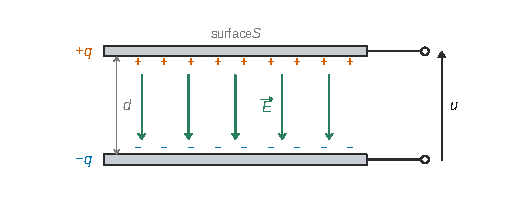
\includegraphics{figures/q01-condensateur-plan.pdf}
\caption*{Figure 1 --- Condensateur plan : charges ±q, champ E uniforme de +q vers
−q, flèche de u vers l'armature +q}
\end{figure}

La flèche de \(u\) va de l'armature \(-q\) vers l'armature \(+q\).

Le champ \(\vec E\), uniforme, va de \(+q\) vers \(-q\).

Il est nul à l'extérieur : les effets de bord sont négligés car \(d\ll\sqrt S\).

\begin{piege}

Le rapport 2026 (p.~89) relève, sur cette question presque toujours réussie, des tensions dessinées comme des vecteurs et des champs ou des flèches de tension orientés à l'envers. La tension est une flèche entre deux armatures, pas un vecteur du champ. Ce schéma fixe tous les signes de la partie : un champ dessiné à l'extérieur ou une flèche de \(u\) vers l'armature négative fausse la suite.

\end{piege}

\hypertarget{question-2}{%
\subsection{Question 2}\label{question-2}}

\begin{indication}{1}

La capacité se définit par une relation de proportionnalité entre deux grandeurs du schéma précédent.

\end{indication}

\begin{indication}{2}

Pour le champ, modéliser chaque armature par un plan infini chargé (hypothèse \(d\ll\sqrt S\)), utiliser symétries et invariances, puis le théorème de Gauss, puis la superposition.

\end{indication}

\begin{indication}{3}

La tension est la circulation du champ d'une armature à l'autre.

\end{indication}

\hypertarget{solution-1}{%
\subsubsection{Solution}\label{solution-1}}

\textbf{1) Définition de la capacité.} Les armatures sont en influence totale. La charge \(q\) de l'armature vers laquelle pointe \(u\) est proportionnelle à \(u\) :
\equationajustee{\boxed{C=\frac{q}{u}}}
C'est un coefficient positif, qui ne dépend que de la géométrie et de l'isolant.

\textbf{2) Détermination du champ.} Pour un plan infini de densité \(\sigma\) et de normale \(\vec n\) :

\begin{itemize}
\tightlist
\item
  tout plan contenant \(\vec n\) est plan de symétrie, donc \(\vec E=E\,\vec n\) ;
\item
  l'invariance par translation dans le plan donne \(E=E(z)\) ;
\item
  le plan chargé est lui-même plan de symétrie, donc \(E(-z)=-E(z)\).
\end{itemize}

Le théorème de Gauss sur un cylindre de section \(\Sigma\) traversant le plan symétriquement donne
\equationajustee{2E(z)\Sigma=\frac{\sigma\Sigma}{\varepsilon_0}}
Le champ d'un plan a donc pour norme \(\sigma/2\varepsilon_0\) ; il s'éloigne du plan si \(\sigma>0\).

On superpose les deux plans, de densités \(\sigma=q/S\) et \(-\sigma\). À l'extérieur, les deux champs sont opposés et s'annulent. Entre les armatures, ils sont tous deux dirigés de \(+q\) vers \(-q\) et s'ajoutent :
\equationajustee{\boxed{\vec E=\frac{q}{\varepsilon_0S}\,\vec u_{+\to-}}}

\textbf{3) Lien entre le champ et la tension.} Le champ étant uniforme sur la distance \(d\) :
\equationajustee{\begin{aligned}
u&=\int_+^-\vec E\cdot\mathrm d\vec\ell\\
&=Ed\\
&=\frac{qd}{\varepsilon_0S}
\end{aligned}}

\textbf{4) Expression de la capacité.} La définition \(C=q/u\) donne
\equationajustee{\boxed{C=\frac{\varepsilon_0S}{d}}}

\begin{methode}

Pour un champ de distribution plane : symétries (direction), invariances (variables), Gauss (norme), superposition. C'est la démarche que l'énoncé demande de « détailler ».

\end{methode}

\begin{jury}

Le rapport 2026 (p.~89) attendait une réponse structurée, avec les résultats intermédiaires mis en évidence : « 1) définition de la capacité, 2) détermination du champ électrique, 3) lien entre le champ et la tension, 4) expression de la capacité ». Il ajoute qu'« il ne fallait pas passer trop de temps sur cette question préliminaire » : une démarche complète tient sur une demi-feuille, sans figure en trois dimensions.

\end{jury}

\hypertarget{question-3}{%
\subsection{Question 3}\label{question-3}}

\begin{indication}{1}

La capacité est proportionnelle à l'aire des surfaces conductrices en regard (question 2, en parallèle).

\end{indication}

\begin{indication}{2}

Lire la figure 1 : à \(\theta_{\mathrm r}=0\), où sont les secteurs clairs (rotor) par rapport aux secteurs sombres (stator) ?

\end{indication}

\hypertarget{solution-2}{%
\subsubsection{Solution}\label{solution-2}}

Les électrodes (1) et (2) sont reliées par l'axe, (3) et (4) entre elles. La capacité est la somme des capacités des zones en regard, donc proportionnelle à l'aire en regard.

\begin{itemize}
\tightlist
\item
  À \(\theta_{\mathrm r}=0\), les électrodes rotoriques occupent les deux quadrants libres : pas de recouvrement, capacité minimale (résiduelle, par effets de bord).
\item
  Après une rotation de \(\pi/2\), chaque électrode rotorique est exactement au-dessus d'une électrode statorique.
\item
  Le motif se répète après une rotation de \(\pi\).
\end{itemize}

\equationajustee{\boxed{\begin{aligned}{}&C_{\min}\ \text{en}\ \theta_{\mathrm r}=k\pi\\
&C_{\max}\ \text{en}\ \theta_{\mathrm r}=\frac{\pi}{2}+k\pi
\end{aligned}}}
La surface en regard maximale est celle de deux quarts de disque, soit \(\pi R^2/2\) (zone de rayon \(\delta\ll R\) négligée). Avec \(d\ll R\) :
\equationajustee{\boxed{C_{\max}=\frac{\pi\varepsilon_0R^2}{2d}}}

\begin{piege}

Oublier qu'il y a deux paires d'électrodes en regard, et trouver \(\pi\varepsilon_0R^2/4d\). Le rapport 2026 note aussi que l'aire d'un disque n'est pas toujours connue.

\end{piege}

\hypertarget{question-4}{%
\subsection{Question 4}\label{question-4}}

\begin{indication}{1}

Exprimer l'aire de recouvrement en fonction de \(\theta_{\mathrm r}\) : l'aire d'un secteur est proportionnelle à son angle.

\end{indication}

\begin{indication}{2}

On peut ensuite raccorder la loi obtenue aux deux valeurs extrêmes, ce qui intègre \(C_{\min}\) sans le calculer.

\end{indication}

\hypertarget{solution-3}{%
\subsubsection{Solution}\label{solution-3}}

Sur \([0,\pi/2]\), chaque électrode rotorique recouvre une électrode statorique sur un secteur d'angle \(\theta_{\mathrm r}\). L'aire en regard vaut \(2\cdot\tfrac12R^2\theta_{\mathrm r}\) : elle est affine en \(\theta_{\mathrm r}\). Sur \([\pi/2,\pi]\), elle décroît symétriquement.
\equationajustee{\boxed{C(\theta_{\mathrm r})=\begin{cases}C_{\min}+\dfrac{2}{\pi}(C_{\max}-C_{\min})\,\theta_{\mathrm r}, & 0\le\theta_{\mathrm r}\le\dfrac{\pi}{2}\\[2mm] C_{\min}+\dfrac{2}{\pi}(C_{\max}-C_{\min})\,(\pi-\theta_{\mathrm r}), & \dfrac{\pi}{2}\le\theta_{\mathrm r}\le\pi\end{cases}}}

Tracé sur \([0,2\pi]\) : triangles de segments droits (première ligne de la figure 2, question 6). \textbf{Période \(\pi\).}

\begin{longtable}[]{@{}
  >{\raggedright\arraybackslash}p{(\columnwidth - 10\tabcolsep) * \real{0.1667}}
  >{\raggedright\arraybackslash}p{(\columnwidth - 10\tabcolsep) * \real{0.1667}}
  >{\raggedright\arraybackslash}p{(\columnwidth - 10\tabcolsep) * \real{0.1667}}
  >{\raggedright\arraybackslash}p{(\columnwidth - 10\tabcolsep) * \real{0.1667}}
  >{\raggedright\arraybackslash}p{(\columnwidth - 10\tabcolsep) * \real{0.1667}}
  >{\raggedright\arraybackslash}p{(\columnwidth - 10\tabcolsep) * \real{0.1667}}@{}}
\toprule\noalign{}
\begin{minipage}[b]{\linewidth}\raggedright
\(\theta_{\mathrm r}\)
\end{minipage} & \begin{minipage}[b]{\linewidth}\raggedright
\(0\)
\end{minipage} & \begin{minipage}[b]{\linewidth}\raggedright
\(\pi/2\)
\end{minipage} & \begin{minipage}[b]{\linewidth}\raggedright
\(\pi\)
\end{minipage} & \begin{minipage}[b]{\linewidth}\raggedright
\(3\pi/2\)
\end{minipage} & \begin{minipage}[b]{\linewidth}\raggedright
\(2\pi\)
\end{minipage} \\
\midrule\noalign{}
\endhead
\bottomrule\noalign{}
\endlastfoot
\(C\) & \(C_{\min}\) & \(C_{\max}\) & \(C_{\min}\) & \(C_{\max}\) & \(C_{\min}\) \\
\end{longtable}

\begin{piege}

Annoncer une période \(2\pi\) : le rotor porte deux électrodes diamétralement opposées, une rotation de \(\pi\) redonne la même configuration.

\end{piege}

\begin{jury}

Le rapport 2026 (p.~89) ouvre son commentaire par « Les difficultés commencent. » Il précise qu'« un très grand nombre d'entre eux ont opté pour une fonction sinusoïdale alors que la réponse attendue était une loi triangulaire périodique variant linéairement par morceau de façon symétrique ». L'erreur a compromis une bonne partie de la suite : la loi se déduit de l'aire en regard, elle ne se devine pas.

\end{jury}

\hypertarget{question-5}{%
\subsection{Question 5}\label{question-5}}

\begin{indication}{1}

Écrire l'énergie électrostatique en fonction de \(C\) et de \(u\), puis dériver à \(u\) fixé.

\end{indication}

\begin{indication}{2}

Pour la tension constante, calculer la moyenne de \(\mathrm dC/\mathrm d\theta_{\mathrm r}\) sur une période : que vaut l'intégrale de la dérivée d'une fonction périodique ?

\end{indication}

\hypertarget{solution-4}{%
\subsubsection{Solution}\label{solution-4}}

L'énergie stockée est \(\mathcal E_{\text{el}}=\tfrac12C(\theta_{\mathrm r})u^2\), donc
\equationajustee{\boxed{\Gamma=\frac12u^2\frac{\mathrm dC}{\mathrm d\theta_{\mathrm r}}}}
Pour un moteur, la puissance moyenne \(\langle\Gamma\rangle\Omega\) fournie à la charge doit être positive : il faut \textbf{\(\langle\Gamma\rangle\neq0\) et du signe de \(\Omega\)}.

Sous \(u=U\) constante :
\equationajustee{\begin{aligned}
\langle\Gamma\rangle&=\frac{U^2}{2\pi}\int_0^\pi\frac{\mathrm dC}{\mathrm d\theta_{\mathrm r}}\,\mathrm d\theta_{\mathrm r}\\
&=\frac{U^2}{2\pi}\big[C(\pi)-C(0)\big]\\
&=0
\end{aligned}}
\textbf{Non} : le couple, du signe de \(\mathrm dC/\mathrm d\theta_{\mathrm r}\), ramène toujours le rotor vers la position de capacité maximale, où il se bloque.

\begin{methode}

Pour tout convertisseur à énergie stockée \(\tfrac12X(\theta)Y^2\) avec \(X\) périodique, une alimentation constante donne un couple moyen nul. L'argument resservira mot pour mot en Q17.

\end{methode}

\begin{piege}

Dériver aussi la tension : la dérivée est prise à \(u\) fixé. Le rapport 2026 (p.~89) le relève : « Certains candidats ont gardé la tension dans la dérivée. »

\end{piege}

\begin{jury}

Le rapport 2026 (p.~89) attend la justification : « Une démonstration rapide utilise le fait que la moyenne sur une période de la dérivée d'une fonction périodique est nulle, mais beaucoup ont donné le résultat sans justification. »

\end{jury}

\hypertarget{question-6}{%
\subsection{Question 6}\label{question-6}}

\begin{indication}{1}

Le couple a le signe de \(\mathrm dC/\mathrm d\theta_{\mathrm r}\) et la tension intervient au carré.

\end{indication}

\begin{indication}{2}

On n'alimente que là où le couple est moteur ; le couple moyen se calcule comme valeur crête × fraction de période.

\end{indication}

\hypertarget{solution-5}{%
\subsubsection{Solution}\label{solution-5}}

Pour \(\Omega>0\), on coupe la tension là où \(C\) décroît :
\equationajustee{\boxed{\begin{aligned}{}&u=U\ \text{sur}\ \Big]k\pi,\ k\pi+\frac{\pi}{2}\Big[\\
&u=0\ \text{sur}\ \Big]k\pi+\frac{\pi}{2},\ (k+1)\pi\Big[
\end{aligned}}}
On note \(\Delta C=C_{\max}-C_{\min}\). Sur les intervalles alimentés, la pente vaut \(2\Delta C/\pi\), donc
\equationajustee{\Gamma=\frac{U^2(C_{\max}-C_{\min})}{\pi}}
Ailleurs, \(\Gamma=0\). La courbe \(\Gamma(\theta_{\mathrm r})\) est un créneau positif de période \(\pi\) et de rapport cyclique \(1/2\), en phase avec les rampes montantes de \(C\) :

\begin{figure}[H]
\centering
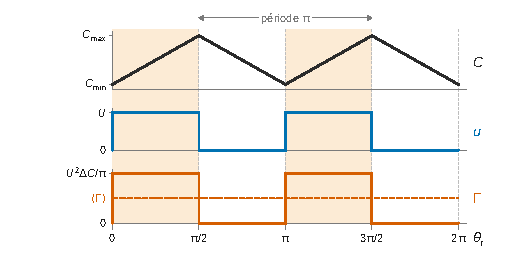
\includegraphics{figures/q06-diagramme-synchrone-capacite.pdf}
\caption*{Figure 2 --- Diagramme synchrone du moteur électrostatique : capacité
C(θr), tension u et couple Γ}
\end{figure}

\equationajustee{\boxed{\langle\Gamma\rangle=\frac{U^2(C_{\max}-C_{\min})}{2\pi}}}

\begin{piege}

Confondre la valeur crête du couple (\(U^2\Delta C/\pi\)) et sa valeur moyenne (\(U^2\Delta C/2\pi\)). Inutile aussi d'imaginer une tension alternative : seul \(u^2\) compte.

\end{piege}

\begin{jury}

Question souvent bien traitée, mais aux explications peu claires ; des candidats « ont été sauvés par le tracé exploité du couple ». Le rapport 2026 (p.~89) conclut : « Un schéma simple et rapidement commenté vaut souvent mieux qu'une longue explication dans laquelle les candidats ont l'habitude de se perdre. »

\end{jury}

\hypertarget{question-7}{%
\subsection{Question 7}\label{question-7}}

\begin{indication}{1}

Après quelle rotation du rotor la séquence d'alimentation doit-elle se répéter ?

\end{indication}

\hypertarget{solution-6}{%
\subsubsection{Solution}\label{solution-6}}

La tension doit reprendre la même valeur chaque fois que le rotor retrouve la même configuration, c'est-à-dire tous les demi-tours. Avec \(\theta_{\mathrm r}=\Omega t\), la période est \(T=\pi/\Omega\), et le fondamental a la période du créneau :
\equationajustee{\boxed{\omega=2\Omega}}

\begin{piege}

Écrire \(\omega=\Omega\) en associant une période électrique à un tour complet. La période de \(C(\theta_{\mathrm r})\) est \(\pi\), pas \(2\pi\).

\end{piege}

\begin{jury}

Le rapport 2026 (p.~89) est net : « La période temporelle du créneau doit correspondre à un demi-tour du rotor. Beaucoup de candidats ne l'ont pas remarqué et cette erreur s'est répercutée en cascade sur l'épreuve. »

\end{jury}

\hypertarget{question-8}{%
\subsection{Question 8}\label{question-8}}

\begin{indication}{1}

En régime permanent, la vitesse est constante : comment relier puissance moyenne et couple moyen ?

\end{indication}

\begin{indication}{2}

Exprimer ensuite \(\Omega\) en fonction de \(f\) grâce à la question 7.

\end{indication}

\hypertarget{solution-7}{%
\subsubsection{Solution}\label{solution-7}}

D'après la question 7, \(f=\Omega/\pi\), soit \(\Omega=\pi f\). La vitesse étant constante, \(\langle\Gamma\Omega\rangle=\langle\Gamma\rangle\Omega\) :
\equationajustee{\begin{aligned}
\langle\mathcal P_{\text{m,el}}\rangle&=\frac{U^2(C_{\max}-C_{\min})}{2\pi}\cdot\pi f\\
&=\boxed{\frac12fU^2(C_{\max}-C_{\min})}
\end{aligned}}

\begin{methode}

Contrôle d'homogénéité : \(\tfrac12U^2\Delta C\) est une énergie, convertie une fois par période électrique ; multipliée par \(f\), c'est une puissance.

\end{methode}

\hypertarget{question-9}{%
\subsection{Question 9}\label{question-9}}

\begin{indication}{1}

Trouver la plus petite rotation qui ramène le motif rotor/stator sur lui-même, et vérifier si la surface rotorique totale dépend de \(p\).

\end{indication}

\begin{indication}{2}

Tout se déduit des questions 6 à 8 en remplaçant la période \(\pi\) par la nouvelle période.

\end{indication}

\hypertarget{solution-8}{%
\subsubsection{Solution}\label{solution-8}}

\textbf{Période.} Les secteurs d'angle \(\pi/2p\), espacés de \(\pi/2p\), forment un motif reproduit après une rotation de \(\pi/p\) :
\equationajustee{\boxed{\text{\text{période} de }C\ :\ \frac{\pi}{p}}}
La surface rotorique, \(2p\cdot\tfrac12R^2\cdot\tfrac{\pi}{2p}\), vaut toujours \(\pi R^2/2\) : \(C_{\max}\) est inchangée.

\textbf{Intervalles.} On alimente là où \(C\) croît :
\equationajustee{\boxed{u=U\ \text{sur}\ \Big]\frac{k\pi}{p},\ \frac{k\pi}{p}+\frac{\pi}{2p}\Big[}}

\textbf{Couple moyen.} La pente devient \(2p\Delta C/\pi\) et le couple crête \(pU^2\Delta C/\pi\), avec un rapport cyclique \(1/2\). Le couple moyen est multiplié par \(p\) :
\equationajustee{\boxed{\langle\Gamma\rangle=\frac{pU^2(C_{\max}-C_{\min})}{2\pi}}}

\textbf{Pulsation.} La période temporelle devient \(\pi/(p\Omega)\) :
\equationajustee{\boxed{\omega=2p\Omega}}

\textbf{Puissance.} Avec \(\Omega=\pi f/p\) :
\equationajustee{\begin{aligned}
\langle\mathcal P\rangle&=\langle\Gamma\rangle\Omega\\
&=\boxed{\frac12fU^2(C_{\max}-C_{\min})}
\end{aligned}}
Elle est \textbf{inchangée à fréquence donnée} : le couple est multiplié par \(p\), la vitesse divisée par \(p\).

\begin{piege}

Conclure « la puissance est multipliée par \(p\) » sans dire ce qu'on garde constant : c'est vrai à \(\Omega\) fixée, faux à \(f\) fixée. Il faut préciser la grandeur maintenue.

\end{piege}

\begin{jury}

Le rapport 2026 (p.~89, commentaire « Q8 ») signale que « Des candidats ont répondu avec \(p=2\) et la généralisation à une valeur quelconque de \(p\) s'est révélée difficile ». Surtout, « le fait que la puissance moyenne restait inchangée a rarement été mis en évidence » : c'est la conclusion attendue, à écrire explicitement.

\end{jury}

\hypertarget{question-10}{%
\subsection{Question 10}\label{question-10}}

\begin{indication}{1}

Compter les espaces inter-plaques sur la figure 2-(c) et se demander à quels potentiels sont toutes les plaques rotoriques, puis toutes les plaques statoriques.

\end{indication}

\begin{indication}{2}

Des condensateurs soumis à la même tension sont en parallèle. Pour l'AN, attention aux unités (mm et µm) et à la consigne d'un chiffre significatif.

\end{indication}

\hypertarget{solution-9}{%
\subsubsection{Solution}\label{solution-9}}

\textbf{Relation.} L'empilement est S--R--S--\ldots--R--S : chaque plaque rotorique est entre deux plaques statoriques, soit \(2N\) espaces d'épaisseur \(d\), chacun équivalent à la structure à une couche.

Toutes les plaques rotoriques sont reliées à l'axe, toutes les statoriques entre elles. Les \(2N\) condensateurs sont soumis à la même tension : ils sont en parallèle.
\equationajustee{\boxed{C_N(\theta_{\mathrm r})=2NC(\theta_{\mathrm r})}}
La puissance moyenne \(\tfrac12fU^2(C_{N,\max}-C_{N,\min})\) est \textbf{multipliée par \(2N\)}.

\textbf{AN} (\(R=10^{-2}\) m, \(d=1{,}5\times10^{-4}\) m ; \(p=3\) ne change pas \(C_{\max}\)) :
\equationajustee{\begin{aligned}
C_{\max}&=\frac{\pi\varepsilon_0R^2}{2d}\\
&=\frac{\pi\times9\times10^{-12}\times10^{-4}}{3\times10^{-4}}\ \text{F}\\
&\approx9\times10^{-12}\ \text{F}
\end{aligned}}
\equationajustee{\boxed{C_{N,\max}=28\,C_{\max}\approx3\times10^{-10}\ \text{F}}}
Avec \(C_{N,\min}\ll C_{N,\max}\), \(U=100\) V et \(f=1\) kHz :
\equationajustee{\langle\mathcal P\rangle\approx\frac12\times10^{3}\times10^{4}\times2{,}6\times10^{-10}\ \text{W}}
\equationajustee{\boxed{\langle\mathcal P\rangle\approx1\ \text{mW}}}

\textbf{Commentaire.} Le moteur occupe environ 4 cm³ (diamètre 2 cm, hauteur d'environ 13 mm). Sa puissance volumique, de l'ordre de \(3\times10^{2}\) W·m⁻³, est ridicule devant celle d'un petit moteur électromagnétique de même volume (de l'ordre du watt).

La vitesse \(\Omega=\pi f/p\approx10^{3}\) rad·s⁻¹ (environ \(10^{4}\) tr/min) est déjà élevée : augmenter \(f\) n'est pas une solution. Le moteur électrostatique macroscopique ne convient qu'aux faibles puissances ; la partie IV explique pourquoi.

\begin{piege}

Compter \(N\), \(N+1\) ou \(2N+1\) condensateurs au lieu de \(2N\). L'épaisseur des plaques (300 µm) n'intervient pas dans la capacité, seulement dans l'encombrement. Et ne pas donner un résultat en « USI » : le rapport 2026 (p.~28) rappelle que ce sigle n'est pas accepté.

\end{piege}

\begin{jury}

Selon le rapport 2026 (p.~89--90, commentaire « Q9 »), « beaucoup n'ont pas observé que les \(2N\) condensateurs soumis à la même tension étaient en parallèle ». Les AN ont donné des puissances « parfois vertigineuses », et « Peu ont conclu que les moteurs électrostatiques ne sont envisageables que pour de faibles puissances. » Un ordre de grandeur vérifié et un commentaire physique sont attendus.

\end{jury}

\hypertarget{question-11}{%
\subsection{Question 11}\label{question-11}}

\begin{indication}{1}

Un conducteur isolé, en influence avec deux autres, joue le rôle de point milieu entre deux condensateurs. Comment sont-ils associés ?

\end{indication}

\begin{indication}{2}

Utiliser une symétrie de la figure 3 pour comparer les deux capacités rotor/demi-stator, puis reprendre la formule de la puissance moyenne.

\end{indication}

\hypertarget{solution-10}{%
\subsubsection{Solution}\label{solution-10}}

\textbf{Schéma équivalent} : entre les demi-stators A et B, deux condensateurs variables en série, \(C_A\) (A--rotor) et \(C_B\) (rotor--B), le rotor flottant étant le point milieu.

\begin{figure}[H]
\centering
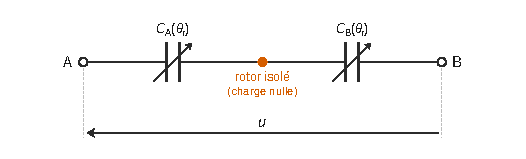
\includegraphics{figures/q11-schema-equivalent-brushless.pdf}
\caption*{Figure 3 --- Schéma équivalent du moteur « brushless » : deux
condensateurs variables en série, rotor isolé au point milieu}
\end{figure}

Dans le montage initial, les deux parties du stator étaient reliées : \(C=C_A+C_B\). La rotation de \(\pi\) laisse le rotor invariant et échange A et B, donc \(C_A=C_B=C/2\) pour tout \(\theta_{\mathrm r}\) :
\equationajustee{\begin{aligned}
C_{\text{\text{éq}}}&=\frac{C_AC_B}{C_A+C_B}\\
&=\frac{C}{4}
\end{aligned}}
Le rotor a une charge fixée (nulle) : l'énergie s'écrit \(\tfrac12C_{\text{\text{éq}}}u^2\), et les questions 5 à 8 s'appliquent avec une excursion \(\Delta C/4\) :
\equationajustee{\langle\mathcal P'\rangle=\frac12fU'^2\,\frac{\Delta C}{4}}
Pour retrouver la même puissance :
\equationajustee{\boxed{U'=2U}}

\begin{piege}

N'utiliser qu'un seul des deux facteurs 2 (série, partage du stator) et trouver \(U'=\sqrt2\,U\).

\end{piege}

\begin{jury}

Question la plus sélective de la partie I. Le rapport 2026 (p.~90, commentaire « Q10 ») écrit : « Cette question a laissé les étudiants perplexes, un nombre très faible y a répondu correctement. » Le schéma équivalent rapporte déjà des points : il faut le proposer, même sans conclure.

\end{jury}

\hypertarget{partie-ii-moteur-uxe9lectromagnuxe9tique-monophasuxe9-uxe0-inductance-variable}{%
\section{Partie II --- Moteur électromagnétique monophasé à inductance variable}\label{partie-ii-moteur-uxe9lectromagnuxe9tique-monophasuxe9-uxe0-inductance-variable}}

On modélise le circuit magnétique (fer de perméabilité infinie, deux entrefers minces) pour obtenir le champ dans l'entrefer par le théorème d'Ampère, puis l'inductance par l'énergie magnétique. Le reste est le décalque magnétique de la partie I.

\hypertarget{question-12}{%
\subsection{Question 12}\label{question-12}}

\begin{indication}{1}

Comparer, à la traversée de l'interface fer/air, le comportement de \(\vec B\) et celui de \(\vec H\).

\end{indication}

\begin{indication}{2}

La composante normale de \(\vec B\) est continue et \(\vec B=\mu_0\mu_{\mathrm r}\vec H\) dans le fer : laquelle des deux grandeurs est grande partout dans le fer, laquelle seulement dans l'entrefer ?

\end{indication}

\hypertarget{solution-11}{%
\subsubsection{Solution}\label{solution-11}}

Dans le fer, \(\vec B=\mu_0\mu_{\mathrm r}\vec H\) avec \(\mu_{\mathrm r}\gg1\) ; dans l'air, \(\vec B=\mu_0\vec H\).

Le champ traverse l'entrefer quasi normalement aux faces polaires, et le flux de \(\vec B\) est conservatif : \(B_n\) est continue. Donc \(\|\vec B\|\) est du même ordre dans le fer et dans l'entrefer, tandis que \(\|\vec H\|\) est \(\mu_{\mathrm r}\) fois plus grand dans l'entrefer.

La simulation 1 est claire (faible) partout sauf dans la mince bande d'entrefer : c'est \(\|\vec H\|\). La simulation 2 est foncée (forte) dans tout le fer parcouru par le flux :
\equationajustee{\boxed{\|\vec B\|\ \text{: simulation 2}}}

\begin{piege}

L'argument « les lignes de champ sont resserrées » ne distingue pas \(B\) de \(H\) : les deux simulations montrent les mêmes lignes. Ce qui les distingue, c'est le saut à l'interface fer/air. Le rapport 2026 (p.~90) met aussi en garde : « Attention, on ne peut pas comparer les intensités de deux grandeurs d'unités différentes (\(H\) et \(B\)). » On compare chaque grandeur d'une région à l'autre.

\end{piege}

\begin{jury}

Le rapport 2026 (p.~90, commentaire « Q11 ») note que les explications ont été « longues et diffuses mais beaucoup ont noté que le flux magnétique était conservatif ». Deux phrases suffisent : conservation du flux, puis lecture des deux cartes.

\end{jury}

\hypertarget{question-13}{%
\subsection{Question 13}\label{question-13}}

\begin{indication}{1}

Commencer par regarder les simulations : où passent les lignes de champ ?

\end{indication}

\begin{indication}{2}

Pour l'expliquer : que vaut \(\vec H\) dans un fer de très grande perméabilité, et où se concentre alors la circulation de \(\vec H\) imposée par le théorème d'Ampère ?

\end{indication}

\hypertarget{solution-12}{%
\subsubsection{Solution}\label{solution-12}}

\textbf{Observation.} Sur la figure 5, les lignes de champ restent canalisées dans le fer (culasse, pôles, rotor) et ne passent dans l'air qu'à la traversée des deux entrefers. Hors des entrefers, presque aucune ligne ne parcourt l'air, et la carte de \(\|\vec B\|\) y est claire : le champ y est négligeable.

\textbf{Interprétation.} Dans le fer, \(\vec H=\vec B/\mu\simeq\vec 0\) : la circulation de \(\vec H\), égale au courant enlacé \(2Ni\), se fait dans l'air.

Un contour passant par les entrefers ne traverse l'air que sur \(2e\). Un contour qui traverse l'air hors des pôles le fait sur une longueur \(2D\), avec \(D\sim R\gg e\). On en déduit les ordres de grandeur
\equationajustee{\begin{aligned}
H_{\text{entrefer}}&\simeq\frac{Ni}{e}\\
H_{\text{air}}&\simeq\frac{Ni}{D}
\end{aligned}}
d'où
\equationajustee{\boxed{\frac{B_{\text{air, hors entrefer}}}{B_{\text{entrefer}}}\sim\frac{e}{D}\ll1}}

\begin{jury}

Le rapport 2026 (p.~90, commentaire « Q12 ») : « Une simple observation des lignes de champ sur ces simulations suffisait pour répondre à cette question ». Des candidats ont perdu du temps dans des démonstrations par le théorème d'Ampère : l'observation d'abord, une ligne d'interprétation ensuite.

\end{jury}

\hypertarget{question-14}{%
\subsection{Question 14}\label{question-14}}

\begin{indication}{1}

Choisir pour contour d'Ampère une ligne de champ passant par les deux entrefers, et l'orienter ; recenser le courant enlacé et chaque contribution à la circulation.

\end{indication}

\begin{indication}{2}

Deux enroulements de \(N\) spires et deux entrefers : les facteurs 2 se compensent-ils ?

\end{indication}

\hypertarget{solution-13}{%
\subsubsection{Solution}\label{solution-13}}

Contour : la ligne de champ pôle statorique → entrefer → rotor → entrefer → pôle opposé → culasse, orientée dans le sens du champ.

\begin{itemize}
\tightlist
\item
  Courant enlacé : \(2Ni\) (deux enroulements en série dont les ampères-tours s'ajoutent).
\item
  Fer (\(\mu\to\infty\), \(B\) fini) : \(\vec H=\vec 0\).
\item
  Chaque entrefer : champ normal aux faces et uniforme (\(e\ll R\)), contribution \(H_ae\).
\end{itemize}

\equationajustee{2H_ae=2Ni}
Avec \(B_a=\mu_0H_a\) dans l'air :
\equationajustee{\boxed{B_a=\frac{\mu_0Ni}{e}}}
en tout point des deux entrefers.

\begin{methode}

Circuit magnétique à fer parfait : la circulation de \(\vec H\) ne « coûte » que dans l'air. La circulation de \(\vec H\) vaut les ampères-tours enlacés, et l'on écrit bien \(\vec H\), pas \(\vec B/\mu_0\), dans le fer.

\end{methode}

\begin{piege}

Confondre ligne de champ et ligne de courant, ou ne pas orienter le contour : le rapport 2026 (p.~90) juge cette confusion « trop fréquente ». Le contour d'Ampère est une ligne de champ magnétique orientée ; le courant enlacé se compte avec la règle de la main droite.

\end{piege}

\begin{jury}

Le rapport 2026 (p.~90, commentaire « Q13 ») : « Disposant du résultat, de nombreux candidats ont tenté de le forcer, quitte à utiliser des raisonnements erronés. » Un résultat donné se démontre : chaque contribution à la circulation doit être écrite.

\end{jury}

\hypertarget{question-15}{%
\subsection{Question 15}\label{question-15}}

\begin{indication}{1}

Placer les pôles sur un cercle : stator centré sur \(\pm\pi/2\), rotor sur \(\theta_{\mathrm r}\) et \(\theta_{\mathrm r}+\pi\), avec leurs demi-ouvertures.

\end{indication}

\begin{indication}{2}

Le volume d'entrefer vaut (angle total de recouvrement) × \(Re\ell\). Comparer la somme des demi-ouvertures d'un pôle rotorique et d'un pôle statorique à l'écart angulaire de leurs axes.

\end{indication}

\hypertarget{solution-14}{%
\subsubsection{Solution}\label{solution-14}}

L'aire d'un secteur circulaire d'angle au sommet \(\alpha\) et de rayon \(R\) est \(\tfrac12\alpha R^2\).

Un secteur d'entrefer d'angle \(\alpha\), entre les rayons \(R\) et \(R+e\), de longueur \(\ell\), a donc pour volume
\equationajustee{\begin{aligned}
V&=\frac{\alpha}{2}\big[(R+e)^2-R^2\big]\ell\\
&\simeq\alpha Re\ell
\end{aligned}}
car \(e\ll R\). Ici \(\alpha\) est l'angle total de recouvrement.

\textbf{\(\theta_{\mathrm r}=k\pi\).} Le pôle rotorique occupe \([-\pi/4-\epsilon,\ \pi/4+\epsilon]\). Le pôle statorique supérieur occupe \([\pi/4+\epsilon/2,\ 3\pi/4-\epsilon/2]\) : le recouvrement vaut \(\epsilon/2\).

Allure : seules les cornes des pôles se font face, en quatre petits secteurs d'ouverture \(\epsilon/2\).
\equationajustee{\boxed{V_{\min}=2\epsilon\,Re\ell}}

\textbf{\(\theta_{\mathrm r}=(2k+1)\pi/2\).} Les pôles sont alignés, et le pôle rotorique (plus large) couvre entièrement le pôle statorique. On a deux secteurs d'ouverture \(\beta_{\mathrm s}\), soit un angle total \(\pi-2\epsilon\), voisin de \(\pi\).
\equationajustee{\boxed{V_{\max}\simeq\pi Re\ell}}

\begin{figure}[H]
\centering
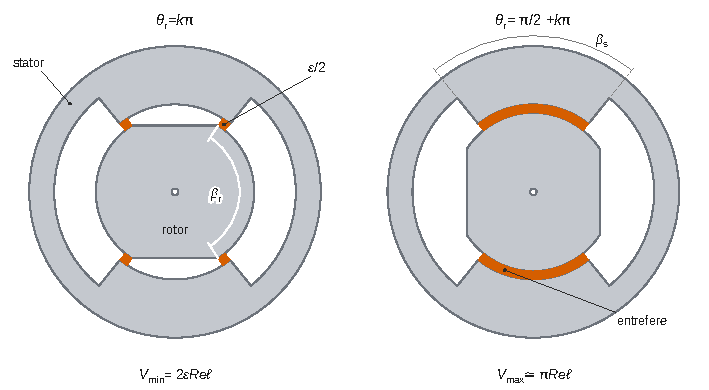
\includegraphics{figures/q15-entrefer-deux-positions.pdf}
\caption*{Figure 4 --- Allure de l'entrefer : quatre coins d'ouverture ε/2 pour θr
= kπ, deux secteurs d'ouverture βs pour θr = π/2 + kπ}
\end{figure}

\begin{piege}

Prendre \(\beta_{\mathrm r}\) au lieu de \(\beta_{\mathrm s}\) pour le recouvrement maximal : c'est le plus étroit des deux pôles qui limite le recouvrement. Et ne pas simplifier \(V_{\min}\) en zéro : \(\epsilon\) y est le seul paramètre angulaire.

\end{piege}

\begin{jury}

Selon le rapport 2026 (p.~90, commentaire « Q14 »), la géométrie a été mal comprise et les schémas trop imprécis : les volumes étaient « le plus souvent faux ». Une intégrale n'est pas nécessaire : « c'était possible plus simplement à condition de connaitre la surface d'un secteur circulaire dont l'angle au sommet est connu ». Un schéma soigné, avec les angles portés, fait la moitié du travail.

\end{jury}

\hypertarget{question-16}{%
\subsection{Question 16}\label{question-16}}

\begin{indication}{1}

L'énergie magnétique d'un circuit parcouru par \(i\) s'écrit avec \(L\) ; il reste à calculer cette énergie à partir du champ.

\end{indication}

\begin{indication}{2}

La densité volumique d'énergie est \(B^2/2\mu\) : où est-elle non négligeable ? Utiliser les questions 13 à 15.

\end{indication}

\begin{indication}{3}

Pour la variation, suivre l'angle de recouvrement quand \(\theta_{\mathrm r}\) va de \(0\) à \(\pi/2\) : combien de zones existent, et comment évolue chacune ?

\end{indication}

\hypertarget{solution-15}{%
\subsubsection{Solution}\label{solution-15}}

\textbf{Définition.} \(\mathcal E_{\text{ma}}\) désignant l'énergie magnétique totale du système :
\equationajustee{\boxed{\mathcal E_{\text{ma}}=\frac12Li^2}}

\textbf{Calcul.} La densité d'énergie \(B^2/2\mu\) est nulle dans le fer (\(\mu\to\infty\)) et négligeable dans l'air hors entrefer. Avec \(B_a=\mu_0Ni/e\) sur le volume \(V\) :
\equationajustee{\mathcal E_{\text{ma}}=\frac{\mu_0N^2i^2}{2e^2}V}
d'où, par identification,
\equationajustee{L=\frac{\mu_0N^2}{e^2}V}
\equationajustee{\boxed{\begin{aligned}
L_{\min}&=\frac{2\mu_0N^2\epsilon R\ell}{e}\\
L_{\max}&=\frac{\pi\mu_0N^2R\ell}{e}
\end{aligned}}}

\textbf{Variation.} \(L\) est proportionnelle à \(\alpha(\theta_{\mathrm r})\) :

\begin{itemize}
\tightlist
\item
  pour \(|\theta_{\mathrm r}|\le\epsilon/2\), deux coins gagnent ce que deux autres perdent : palier à \(L_{\min}\) ;
\item
  pour \(\epsilon/2\le\theta_{\mathrm r}\le\pi/2-3\epsilon/2\), deux zones seulement, croissant chacune comme \(\theta_{\mathrm r}\) : \(\alpha=2\theta_{\mathrm r}+\epsilon\) ;
\item
  puis palier à \(L_{\max}\) tant que le pôle statorique est couvert, et décroissance symétrique.
\end{itemize}

\textbf{\(L\) est affine par morceaux (trapézoïdale), de période \(\pi\)}, ce que confirme la figure 6.

\begin{piege}

Écrire \(B^2/2\mu_0\) dans le fer : on trouverait une énergie dominée par le fer. C'est \(\mu\to\infty\) qui annule la densité d'énergie dans le fer, alors que \(B\) y est du même ordre que dans l'entrefer.

\end{piege}

\begin{piege}

Répondre « \(L\) varie continûment » : la question attend la forme de la variation, linéaire sur chaque rampe. Le rapport 2026 (p.~90, commentaire « Q15 ») le relève : « De nombreux candidats semblent confondre évolution linéaire et évolution continue. »

\end{piege}

\hypertarget{question-17}{%
\subsection{Question 17}\label{question-17}}

\begin{indication}{1}

Même démarche qu'en question 5, avec l'énergie magnétique dérivée à courant fixé.

\end{indication}

\hypertarget{solution-16}{%
\subsubsection{Solution}\label{solution-16}}

\equationajustee{\boxed{\Gamma=\frac12i^2\frac{\mathrm dL}{\mathrm d\theta_{\mathrm r}}}}
À \(i=I\) constant, par périodicité :
\equationajustee{\begin{aligned}
\langle\Gamma\rangle&=\frac{I^2}{2\pi}\big[L(\pi)-L(0)\big]\\
&=0
\end{aligned}}
\textbf{Non}, un courant constant ne fait pas un moteur : le rotor s'immobilise pôles alignés (\(L\) maximale).

\hypertarget{question-18}{%
\subsection{Question 18}\label{question-18}}

\begin{indication}{1}

Repérer sur la figure 6 les rampes montantes, les paliers (largeur \(\Delta\beta\) centrés sur les multiples de \(\pi/2\)) et les rampes descendantes.

\end{indication}

\begin{indication}{2}

Pour le couple moyen, \(\frac{\mathrm dL}{\mathrm d\theta_{\mathrm r}}\mathrm d\theta_{\mathrm r}=\mathrm dL\) : la largeur des paliers intervient-elle ?

\end{indication}

\hypertarget{solution-17}{%
\subsubsection{Solution}\label{solution-17}}

On n'envoie le courant que pendant les rampes montantes de \(L\) :
\equationajustee{\boxed{\begin{aligned}{}&i=I\ \text{sur}\ \Big[k\pi+\frac{\Delta\beta}{2},\ k\pi+\frac{\pi}{2}-\frac{\Delta\beta}{2}\Big]\\
&i=0\ \text{ailleurs}
\end{aligned}}}

Diagramme synchrone, avec la pente de la question 23 :
\equationajustee{\rho=\frac{L_{\max}-L_{\min}}{\pi/2-\Delta\beta}}

\begin{figure}[H]
\centering
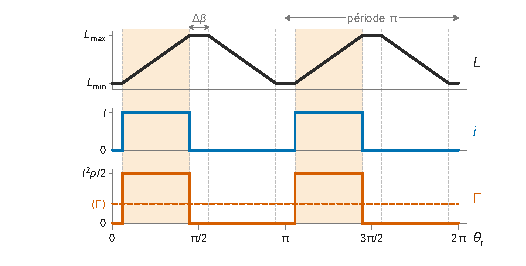
\includegraphics{figures/q18-diagramme-synchrone-inductance.pdf}
\caption*{Figure 5 --- Diagramme synchrone du moteur à inductance variable :
inductance L(θr), courant i et couple Γ}
\end{figure}

Valeurs sur une période (à répéter sur \([\pi,2\pi]\)) :

\begin{longtable}[]{@{}
  >{\raggedright\arraybackslash}p{(\columnwidth - 10\tabcolsep) * \real{0.1019}}
  >{\raggedright\arraybackslash}p{(\columnwidth - 10\tabcolsep) * \real{0.1201}}
  >{\raggedright\arraybackslash}p{(\columnwidth - 10\tabcolsep) * \real{0.1846}}
  >{\raggedright\arraybackslash}p{(\columnwidth - 10\tabcolsep) * \real{0.2215}}
  >{\raggedright\arraybackslash}p{(\columnwidth - 10\tabcolsep) * \real{0.2081}}
  >{\raggedright\arraybackslash}p{(\columnwidth - 10\tabcolsep) * \real{0.1338}}@{}}
\toprule\noalign{}
\begin{minipage}[b]{\linewidth}\raggedright
\(\theta_{\mathrm r}\)
\end{minipage} & \begin{minipage}[b]{\linewidth}\raggedright
\([0,\frac{\Delta\beta}{2}]\)
\end{minipage} & \begin{minipage}[b]{\linewidth}\raggedright
\([\frac{\Delta\beta}{2},\frac{\pi}{2}-\frac{\Delta\beta}{2}]\)
\end{minipage} & \begin{minipage}[b]{\linewidth}\raggedright
\([\frac{\pi}{2}-\frac{\Delta\beta}{2},\allowbreak \frac{\pi}{2}+\frac{\Delta\beta}{2}]\)
\end{minipage} & \begin{minipage}[b]{\linewidth}\raggedright
\([\frac{\pi}{2}+\frac{\Delta\beta}{2},\allowbreak \pi-\frac{\Delta\beta}{2}]\)
\end{minipage} & \begin{minipage}[b]{\linewidth}\raggedright
\([\pi-\frac{\Delta\beta}{2},\pi]\)
\end{minipage} \\
\midrule\noalign{}
\endhead
\bottomrule\noalign{}
\endlastfoot
\(L\) & \(L_{\min}\) & rampe montante & \(L_{\max}\) & rampe descendante & \(L_{\min}\) \\
\(i\) & \(0\) & \(I\) & \(0\) & \(0\) & \(0\) \\
\(\Gamma\) & \(0\) & \(\dfrac{I^2(L_{\max}-L_{\min})}{2(\pi/2-\Delta\beta)}\) & \(0\) & \(0\) & \(0\) \\
\end{longtable}

\equationajustee{\begin{aligned}
\langle\Gamma\rangle&=\frac{I^2}{2\pi}\int_{L_{\min}}^{L_{\max}}\mathrm dL\\
&=\boxed{\frac{I^2(L_{\max}-L_{\min})}{2\pi}}
\end{aligned}}

\begin{methode}

Contrôle croisé : couple crête × rapport cyclique, soit \(\dfrac{I^2\Delta L}{2(\pi/2-\Delta\beta)}\times\dfrac{\pi/2-\Delta\beta}{\pi}\), redonne le même résultat.

\end{methode}

\begin{piege}

Laisser des angles en degrés au dénominateur (« 90° » au lieu de \(\pi/2\)). Le rapport 2026 (p.~90, commentaire « Q17 ») insiste : « il est indispensable d'utiliser les radians dans les calculs littéraux, l'emploi des degrés conduisant à des résultats numériques erronés ».

\end{piege}

\hypertarget{question-19}{%
\subsection{Question 19}\label{question-19}}

\begin{indication}{1}

Quelle est la période angulaire de \(L\), donc du créneau de courant ?

\end{indication}

\hypertarget{solution-18}{%
\subsubsection{Solution}\label{solution-18}}

\(L\) et le créneau sont \(\pi\)-périodiques en \(\theta_{\mathrm r}=\Omega t\), donc \(T=\pi/\Omega\) :
\equationajustee{\boxed{\omega=2\Omega}}

\begin{piege}

Même erreur qu'en question 7 : associer une période à un tour complet et écrire \(\omega=\Omega\). Le rapport 2026 (p.~90) signale ici les mêmes difficultés.

\end{piege}

\hypertarget{question-20}{%
\subsection{Question 20}\label{question-20}}

\begin{indication}{1}

Reprendre exactement la chaîne de la question 8.

\end{indication}

\hypertarget{solution-19}{%
\subsubsection{Solution}\label{solution-19}}

On a \(\Omega=\pi f\), et \(\Omega\) est constante :
\equationajustee{\begin{aligned}
\langle\mathcal P_{\text{m,ma}}\rangle&=\langle\Gamma\rangle\Omega\\
&=\frac{I^2\Delta L}{2\pi}\,\pi f\\
&=\boxed{\frac12fI^2(L_{\max}-L_{\min})}
\end{aligned}}
Même structure qu'en Q8 : l'énergie \(\tfrac12I^2\Delta L\) est convertie une fois par période.

\hypertarget{partie-iii-alimentation-uxe9lectrique-du-moteur-monophasuxe9-uxe0-inductance-variable}{%
\section{Partie III --- Alimentation électrique du moteur monophasé à inductance variable}\label{partie-iii-alimentation-uxe9lectrique-du-moteur-monophasuxe9-uxe0-inductance-variable}}

On écrit l'équation électrique d'une bobine dont l'inductance dépend de la position, puis on analyse deux convertisseurs continu--continu chargés de fabriquer le créneau de courant. Tout repose sur la continuité du courant dans une inductance et sur l'état des interrupteurs.

\hypertarget{question-21}{%
\subsection{Question 21}\label{question-21}}

\begin{indication}{1}

Loi de Faraday avec le flux propre \(\Phi=Li\) ; ici \(L\) dépend du temps par l'intermédiaire de \(\theta_{\mathrm r}\).

\end{indication}

\begin{indication}{2}

Dériver un produit, puis passer de \(\mathrm d/\mathrm dt\) à \(\mathrm d/\mathrm d\theta_{\mathrm r}\).

\end{indication}

\hypertarget{solution-20}{%
\subsubsection{Solution}\label{solution-20}}

En convention récepteur :
\equationajustee{\begin{aligned}
u&=ri+\frac{\mathrm d(Li)}{\mathrm dt}\\
&=ri+L\frac{\mathrm di}{\mathrm dt}+i\frac{\mathrm dL}{\mathrm d\theta_{\mathrm r}}\frac{\mathrm d\theta_{\mathrm r}}{\mathrm dt}
\end{aligned}}
On pose
\equationajustee{\boxed{\Omega=\frac{\mathrm d\theta_{\mathrm r}}{\mathrm dt}}}
et l'on utilise \(\mathrm di/\mathrm dt=\Omega\,\mathrm di/\mathrm d\theta_{\mathrm r}\) :
\equationajustee{\boxed{\Big[r+\Omega\frac{\mathrm dL}{\mathrm d\theta_{\mathrm r}}\Big]i+\Omega L(\theta_{\mathrm r})\frac{\mathrm di}{\mathrm d\theta_{\mathrm r}}=u(\theta_{\mathrm r})}}

\begin{methode}

Contrôle énergétique : en multipliant par \(i\), on obtient
\equationajustee{ui=ri^2+\frac{\mathrm d}{\mathrm dt}\Big(\frac12Li^2\Big)+\frac12i^2\frac{\mathrm dL}{\mathrm d\theta_{\mathrm r}}\Omega}
soit pertes Joule, variation d'énergie stockée et puissance mécanique \(\Gamma\Omega\), en accord avec Q17.

\end{methode}

\begin{piege}

Écrire \(u=ri+L\,\mathrm di/\mathrm dt\) : c'est la loi d'une inductance fixe, elle fait disparaître le terme de conversion.

\end{piege}

\hypertarget{question-22}{%
\subsection{Question 22}\label{question-22}}

\begin{indication}{1}

Un interrupteur idéal fermé impose une tension nulle à ses bornes ; en déduire le potentiel du point commun, puis la tension aux bornes de la diode.

\end{indication}

\begin{indication}{2}

Lire sur la figure 7 le sens de la diode ; pour les règles d'interconnexion, se demander quel dipôle se comporte comme une source de courant.

\end{indication}

\hypertarget{solution-21}{%
\subsubsection{Solution}\label{solution-21}}

T passant relie le point commun K à la borne \(+\) : \(V_K=U_0\), la borne \(-\) étant prise comme référence.

D a son anode à la borne \(-\) et sa cathode en K : la tension à ses bornes vaut \(-U_0<0\), \textbf{D est bloquée}. Le moteur est directement aux bornes de la source :
\equationajustee{\boxed{u=U_0}}
Le transistor est unidirectionnel : \textbf{\(i\ge0\)}, et le courant croît depuis \(0\) sous \(u>0\).

Règles : ne jamais court-circuiter une source de tension, ne jamais ouvrir une source de courant. Par son inductance, le moteur impose la continuité de son courant : c'est un dipôle de type source de courant. La source \(U_0\) alimente donc une source de courant, et D bloquée ne la court-circuite pas : \textbf{règles respectées}.

\begin{jury}

Le rapport 2026 (p.~90, commentaire « Q21 ») demande le vocabulaire « passante/bloquée (à privilégier) » plutôt que fermée/ouverte ou allumée/éteinte. Le point le moins cité était pourtant essentiel : « la présence de l'inductance \(L\) fait du moteur un dipôle de type source de courant qui en garantit la continuité ».

\end{jury}

\hypertarget{question-23}{%
\subsection{Question 23}\label{question-23}}

\begin{indication}{1}

Sur quel intervalle angulaire T est-il commandé ? Lire sur la figure 6 la variation de \(L\) et la largeur de cet intervalle.

\end{indication}

\begin{indication}{2}

Reporter la pente et la valeur de \(u\) dans l'équation de la question 21.

\end{indication}

\hypertarget{solution-22}{%
\subsubsection{Solution}\label{solution-22}}

T conduit sur les intervalles de la question 18, c'est-à-dire sur la rampe montante.

Celle-ci va de la fin du palier bas (\(\Delta\beta/2\)) au début du palier haut (\(\pi/2-\Delta\beta/2\)) ; son amplitude est \(\pi/2-\Delta\beta\). Sur cette rampe, \(L\) passe linéairement de \(L_{\min}\) à \(L_{\max}\), d'où la pente constante
\equationajustee{\frac{\mathrm dL}{\mathrm d\theta_{\mathrm r}}=\frac{L_{\max}-L_{\min}}{\pi/2-\Delta\beta}}
notée \(\rho\). Avec \(u=U_0\) :
\equationajustee{\boxed{(r+\Omega\rho)\,i+\Omega L(\theta_{\mathrm r})\frac{\mathrm di}{\mathrm d\theta_{\mathrm r}}=U_0}}

\begin{piege}

Le dénominateur est \(\pi/2\) diminué de deux demi-paliers, soit \(\pi/2-\Delta\beta\), ni \(\pi/2-\Delta\beta/2\) ni \(\pi/2\). Employer la notation \(\rho\) imposée par l'énoncé.

\end{piege}

\hypertarget{question-24}{%
\subsection{Question 24}\label{question-24}}

\begin{indication}{1}

Le courant d'un dipôle inductif ne peut pas s'interrompre : quel chemin trouve-t-il quand T s'ouvre ?

\end{indication}

\begin{indication}{2}

Découper l'intervalle demandé selon les paliers et la rampe de la figure 6, puis écrire l'équation de Q21 avec la bonne valeur de \(u\).

\end{indication}

\hypertarget{solution-23}{%
\subsubsection{Solution}\label{solution-23}}

À l'ouverture de T (\(\theta_{\mathrm r}=\pi/2-\Delta\beta/2\)), le courant \(i>0\) continue de circuler et se referme par D, dans son sens passant : \textbf{D est passante}, et \(u=0\).

La dérivée \(\mathrm dL/\mathrm d\theta_{\mathrm r}\) vaut successivement :

\begin{itemize}
\tightlist
\item
  \(0\) sur le palier \(L_{\max}\) ;
\item
  \(-\rho\) sur la rampe descendante ;
\item
  \(0\) sur le palier \(L_{\min}\).
\end{itemize}

\equationajustee{\boxed{\begin{aligned}{}&\Big[\tfrac{\pi}{2}-\tfrac{\Delta\beta}{2},\ \tfrac{\pi}{2}+\tfrac{\Delta\beta}{2}\Big] : && r\,i+\Omega L_{\max}\frac{\mathrm di}{\mathrm d\theta_{\mathrm r}}=0\\
&\Big[\tfrac{\pi}{2}+\tfrac{\Delta\beta}{2},\ \pi-\tfrac{\Delta\beta}{2}\Big] : && (r-\Omega\rho)\,i+\Omega L(\theta_{\mathrm r})\frac{\mathrm di}{\mathrm d\theta_{\mathrm r}}=0\\
&\Big[\pi-\tfrac{\Delta\beta}{2},\ \pi+\tfrac{\Delta\beta}{2}\Big] : && r\,i+\Omega L_{\min}\frac{\mathrm di}{\mathrm d\theta_{\mathrm r}}=0
\end{aligned}}}
avec, sur la rampe,
\equationajustee{L(\theta_{\mathrm r})=L_{\max}-\rho\Big(\theta_{\mathrm r}-\frac{\pi}{2}-\frac{\Delta\beta}{2}\Big)}

\begin{piege}

Oublier le palier bas : l'intervalle imposé va jusqu'à \(\pi+\Delta\beta/2\), il contient trois sous-domaines. Et ne pas inverser les paliers : T s'ouvre quand \(L\) atteint \(L_{\max}\), donc la première phase se fait à \(L=L_{\max}\) et la troisième à \(L=L_{\min}\) (figure 6).

\end{piege}

\begin{jury}

Le rapport 2026 (p.~90, commentaire « Q23 ») confirme que la diode est passante et regrette que « Les trois phases à examiner, l'ont été de manière désordonnée ». Il attendait qu'on remplace \(L(\theta_{\mathrm r})\) par sa valeur constante sur chaque palier, ce qui a été rarement fait. Attention : le rapport écrit \(L_{\min}\) pour la première phase et \(L_{\max}\) pour la troisième, ce qui contredit la figure 6 et l'énoncé ; l'ordre correct est celui de la solution ci-dessus.

\end{jury}

\hypertarget{question-25}{%
\subsection{Question 25}\label{question-25}}

\begin{indication}{1}

Isoler \(\mathrm di/\mathrm d\theta_{\mathrm r}\) dans l'équation de Q21 et regarder, phase par phase, le signe et la taille du numérateur et du dénominateur.

\end{indication}

\begin{indication}{2}

Comparer les « constantes d'angle » \(\Omega L/r\) sur les deux paliers, et le rôle du terme \(\Omega\,\mathrm dL/\mathrm d\theta_{\mathrm r}\) selon le signe de la pente.

\end{indication}

\hypertarget{solution-24}{%
\subsubsection{Solution}\label{solution-24}}

\equationajustee{\frac{\mathrm di}{\mathrm d\theta_{\mathrm r}}=\frac{u-(r+\Omega\,\mathrm dL/\mathrm d\theta_{\mathrm r})\,i}{\Omega L}}

\begin{itemize}
\tightlist
\item
  \textbf{Montée} : \(i=0\) et \(L=L_{\min}\) ; la pente \(U_0/(\Omega L_{\min})\) est la plus forte du cycle : front raide.
\item
  \textbf{Plateau} : \((r+\Omega\rho)i\) croît et \(L\) augmente ; \(i\) tend vers \(U_0/(r+\Omega\rho)\) : courant presque constant.
\item
  \textbf{Palier \(L_{\max}\), T ouvert} : décroissance exponentielle de constante d'angle \(\Omega L_{\max}/r\) ; l'énergie n'est dissipée que dans \(r\).
\item
  \textbf{Rampe descendante} : le coefficient devient \(r-\Omega\rho<r\). La machine fonctionne en génératrice et entretient le courant : la décroissance est plus lente encore.
\item
  \textbf{Palier \(L_{\min}\)} : la constante d'angle \(\Omega L_{\min}/r\) est beaucoup plus petite. Le courant résiduel chute plus vite, juste avant l'impulsion suivante (figure 8, vers \(180^\circ\)).
\end{itemize}

\begin{methode}

Une équation du premier ordre en \(\theta_{\mathrm r}\) se lit comme en régime transitoire : la « constante de temps » est ici une constante d'angle, \(\Omega L/(r+\Omega\,\mathrm dL/\mathrm d\theta_{\mathrm r})\). Plus elle est grande devant la largeur angulaire de la phase, plus le courant varie lentement.

\end{methode}

\begin{jury}

Le rapport 2026 (p.~90, commentaire « Q24 ») attendait que l'on repère dans l'équation une constante de relaxation angulaire, du type \(L\Omega/r\), qui contrôle l'évolution du courant : « Rares sont les candidats qui l'ont observé, l'analyse du diagramme a été descriptive, peu ou mal interprétée. » Décrire la courbe ne suffit pas : il faut la relier à l'équation.

\end{jury}

\hypertarget{question-26}{%
\subsection{Question 26}\label{question-26}}

\begin{indication}{1}

Regarder la courbe de couple de la figure 8 : où le couple est-il négatif, et pourquoi y a-t-il encore du courant à cet endroit ?

\end{indication}

\begin{indication}{2}

Quelles valeurs de tension le montage 1 peut-il appliquer au moteur ?

\end{indication}

\hypertarget{solution-25}{%
\subsubsection{Solution}\label{solution-25}}

\textbf{Défaut} : le courant subsiste pendant la rampe descendante de \(L\), où le couple est négatif :
\equationajustee{\Gamma=\frac12i^2\frac{\mathrm dL}{\mathrm d\theta_{\mathrm r}}<0}
C'est un \textbf{couple de freinage}, qui diminue couple moyen et puissance.

\textbf{Cause} : en roue libre, D impose \(u=0\). L'énergie magnétique n'est évacuée que par effet Joule dans la faible résistance \(r\), d'où une extinction lente, encore freinée par le fonctionnement en génératrice. \textbf{Le montage ne peut pas appliquer de tension négative} pour annuler rapidement le courant.

\begin{piege}

Invoquer des pertes dans la diode : elle est idéale. Le défaut à citer est le couple négatif, et sa cause structurelle est l'absence de tension négative.

\end{piege}

\begin{jury}

Question bien réussie, mais mal formulée. La réponse attendue tient en une phrase du rapport 2026 (p.~90--91, commentaire « Q25 ») : le montage « produit un couple négatif parce qu'on continue à envoyer un courant alors que l'inductance décroit ».

\end{jury}

\hypertarget{question-27}{%
\subsection{Question 27}\label{question-27}}

\begin{indication}{1}

Partir de la continuité de \(i>0\) : par quels composants le courant peut-il passer dans chaque phase ?

\end{indication}

\begin{indication}{2}

En déduire les potentiels des deux bornes du moteur, puis vérifier le signe de la tension aux bornes de chaque diode supposée bloquée.

\end{indication}

\hypertarget{solution-26}{%
\subsubsection{Solution}\label{solution-26}}

Notations : H et B sont les bornes \(+\) et \(-\) de la source.

A est le point commun à \(\mathrm T_1\), à \(\mathrm D_1\) et au moteur ; A' le point commun au moteur, à \(\mathrm D_2\) et à \(\mathrm T_2\).

On oriente \(u=V_A-V_{A'}\) et \(i>0\) de A vers A'. \(\mathrm D_1\) a son anode en B et sa cathode en A ; \(\mathrm D_2\) a son anode en A' et sa cathode en H.

\begin{longtable}[]{@{}
  >{\raggedright\arraybackslash}p{(\columnwidth - 8\tabcolsep) * \real{0.2885}}
  >{\raggedright\arraybackslash}p{(\columnwidth - 8\tabcolsep) * \real{0.3016}}
  >{\raggedright\arraybackslash}p{(\columnwidth - 8\tabcolsep) * \real{0.0880}}
  >{\raggedright\arraybackslash}p{(\columnwidth - 8\tabcolsep) * \real{0.1459}}
  >{\raggedright\arraybackslash}p{(\columnwidth - 8\tabcolsep) * \real{0.1459}}@{}}
\toprule\noalign{}
\begin{minipage}[b]{\linewidth}\raggedright
Phase
\end{minipage} & \begin{minipage}[b]{\linewidth}\raggedright
Chemin du courant
\end{minipage} & \begin{minipage}[b]{\linewidth}\raggedright
\(u\)
\end{minipage} & \begin{minipage}[b]{\linewidth}\raggedright
\(\mathrm D_1\)
\end{minipage} & \begin{minipage}[b]{\linewidth}\raggedright
\(\mathrm D_2\)
\end{minipage} \\
\midrule\noalign{}
\endhead
\bottomrule\noalign{}
\endlastfoot
1 : \(\mathrm T_1\), \(\mathrm T_2\) passants & H → \(\mathrm T_1\) → moteur → \(\mathrm T_2\) → B & \(+U_0\) & bloquée & bloquée \\
2 : \(\mathrm T_1\), \(\mathrm T_2\) ouverts & B → \(\mathrm D_1\) → moteur → \(\mathrm D_2\) → H & \(-U_0\) & passante & passante \\
3 : \(\mathrm T_2\) passant, \(\mathrm T_1\) ouvert & moteur → \(\mathrm T_2\) → B → \(\mathrm D_1\) → moteur & \(0\) & passante & bloquée \\
\end{longtable}

En phase 1, chaque diode a une tension \(-U_0\) à ses bornes. En phase 2, le courant entre dans la source par sa borne \(+\) : l'énergie est renvoyée à la source. En phase 3, \(\mathrm D_2\) a la tension \(V_{A'}-V_H=-U_0\) à ses bornes.

Ces états supposent \(i>0\) ; une fois le courant nul, toutes les diodes se bloquent et \(u=0\).

\begin{figure}[H]
\centering
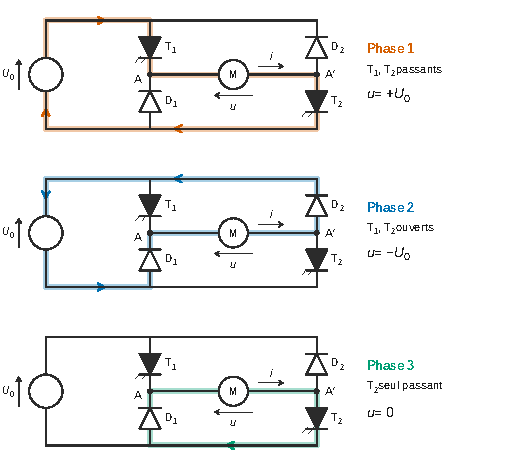
\includegraphics{figures/q27-montage-2-trois-phases.pdf}
\caption*{Figure 6 --- Montage n°2 : chemin du courant et tension u dans les
phases 1, 2 et 3}
\end{figure}

\begin{piege}

Annoncer \(u=0\) en phase 2 : c'est justement \(-U_0\) qui fait l'intérêt du montage. Le montage est réversible en tension, pas en courant (\(i\) reste positif).

\end{piege}

\begin{jury}

Le rapport 2026 (p.~91, commentaire « Q26 ») salue les copies où « certains ont eu la bonne idée de présenter les résultats dans un tableau ». Trois phases et trois grandeurs : le tableau est la présentation naturelle.

\end{jury}

\hypertarget{question-28}{%
\subsection{Question 28}\label{question-28}}

\begin{indication}{1}

Comparer les figures 8 et 10 pendant l'extinction du courant : quelle tension est appliquée, et le courant est-il encore non nul quand \(L\) décroît ?

\end{indication}

\begin{indication}{2}

Penser à deux critères de performance : le couple moyen et le devenir de l'énergie magnétique stockée.

\end{indication}

\hypertarget{solution-27}{%
\subsubsection{Solution}\label{solution-27}}

\textbf{Comparaison.} Les montées sont identiques. À l'extinction, le montage 1 impose \(u=0\) : la décroissance est exponentielle, lente, et s'étend sur toute la rampe descendante.

Le montage 2 impose \(u=-U_0\), d'où \(\Omega L\,\mathrm di/\mathrm d\theta_{\mathrm r}\simeq-U_0\). La décroissance est quasi linéaire et rapide : sur la figure 10, le courant s'annule vers la fin du palier \(L_{\max}\), avant que \(L\) ne décroisse.

\textbf{Performances du montage 2.}

\begin{itemize}
\tightlist
\item
  Plus de courant pendant la décroissance de \(L\) : \textbf{plus de couple de freinage}. Le couple est un créneau positif ; couple moyen et puissance sont proches de l'idéal \(I^2\Delta L/2\pi\).
\item
  L'énergie magnétique est \textbf{renvoyée à la source} (phase 2) au lieu d'être dissipée dans \(r\) : meilleur rendement.
\item
  La phase 3 (roue libre) permet en outre de réguler le courant par découpage.
\end{itemize}

\hypertarget{partie-iv-comparaison-des-deux-types-de-moteurs.-lois-duxe9chelle-et-downsizing}{%
\section{Partie IV --- Comparaison des deux types de moteurs. Lois d'échelle et « downsizing »}\label{partie-iv-comparaison-des-deux-types-de-moteurs.-lois-duxe9chelle-et-downsizing}}

On réécrit les deux puissances sous la forme « densité d'énergie du champ × volume actif × fréquence », on compare les champs limites (claquage de l'air, saturation du fer), puis on suit l'évolution des performances quand toutes les dimensions sont multipliées par \(h\).

\hypertarget{question-29}{%
\subsection{Question 29}\label{question-29}}

\begin{indication}{1}

Exprimer \(U\) en fonction du champ et \(C_{\max}\) en fonction d'un volume ; de même \(I\) en fonction de \(B_e\) et \(L_{\max}\) en fonction de \(V_{e,\max}\).

\end{indication}

\begin{indication}{2}

Résultats utiles : \(E=U/d\) (Q2), \(C=\varepsilon_0S/d\), \(B=\mu_0NI/e\) (Q14), \(L=\mu_0N^2V/e^2\) (Q16).

\end{indication}

\hypertarget{solution-28}{%
\subsubsection{Solution}\label{solution-28}}

\textbf{Électrostatique.} Comme \(C_{\min}\ll C_{\max}\), \(\langle\mathcal P_{\text{m,el}}\rangle\simeq\tfrac12fU^2C_{\max}\). On remplace \(U=E_ad\) et \(C_{\max}\), avec \(V_{a,\max}=S_{\max}d\) :
\equationajustee{C_{\max}=\frac{\varepsilon_0V_{a,\max}}{d^2}}
\equationajustee{\boxed{\langle\mathcal P_{\text{m,el}}\rangle\simeq\frac{\varepsilon_0}{2}fV_{a,\max}E_a^2}}

\textbf{Électromagnétique.} Comme \(L_{\min}\ll L_{\max}\), \(\langle\mathcal P_{\text{m,ma}}\rangle\simeq\tfrac12fI^2L_{\max}\). Avec \(I=B_ee/(\mu_0N)\) et \(L_{\max}=\mu_0N^2V_{e,\max}/e^2\) :
\equationajustee{I^2L_{\max}=\frac{B_e^2V_{e,\max}}{\mu_0}}
\equationajustee{\boxed{\langle\mathcal P_{\text{m,ma}}\rangle\simeq\frac{1}{2\mu_0}fV_{e,\max}B_e^2}}

\begin{methode}

\(\tfrac12\varepsilon_0E^2\) et \(B^2/2\mu_0\) sont les densités d'énergie électrique et magnétique : un convertisseur à énergie stockée fournit \(\langle\mathcal P\rangle\sim f\times\) (énergie du champ dans le volume actif).

\end{methode}

\begin{jury}

Le rapport 2026 (p.~91, commentaire « Q28 ») : « Les résultats étant donnés, beaucoup y sont parvenus (pas toujours avec la plus grande honnêteté). » Chaque substitution doit apparaître ; un passage escamoté vers un résultat fourni ne rapporte rien.

\end{jury}

\hypertarget{question-30}{%
\subsection{Question 30}\label{question-30}}

\begin{indication}{1}

Égaler les deux puissances à volumes et fréquence égaux, puis reconnaître la combinaison \(\varepsilon_0\mu_0\).

\end{indication}

\hypertarget{solution-29}{%
\subsubsection{Solution}\label{solution-29}}

À volumes et fréquence égaux, l'égalité des puissances s'écrit
\equationajustee{\frac{\varepsilon_0}{2}E_a^2=\frac{B_e^2}{2\mu_0}}
Avec \(\varepsilon_0\mu_0c^2=1\), on obtient \(E_a=cB_e\) ; le fer sature à \(B_{\text{sat}}\approx1\) T :
\equationajustee{\boxed{E_a\approx cB_{\text{sat}}\approx3\times10^{8}\ \text{V}\cdot\text{m}^{-1}}}
C'est cinquante à cent fois le champ que l'air peut supporter (Q31).

\begin{piege}

Le rapport 2026 (p.~91, commentaire « Q29 ») relève deux erreurs. D'abord, « Dans l'expression littérale finale, remplacer \(B_{sat}\) par 1 (\(T\)) en gardant \(E_{air}\) est incorrecte » : l'expression littérale reste \(E_a=cB_{\text{sat}}\), la valeur numérique vient ensuite. Ensuite, l'unité : « L'unité d'un champ électrique est à connaitre », ici le V·m⁻¹.

\end{piege}

\hypertarget{question-31}{%
\subsection{Question 31}\label{question-31}}

\begin{indication}{1}

À pression atmosphérique, choisir une distance \(d\) (par exemple 1 mm), en déduire l'abscisse \(pd\), lire \(V_c\) et former \(V_c/d\).

\end{indication}

\begin{indication}{2}

Écrire \(\kappa\) comme le rapport des deux densités d'énergie maximales et faire apparaître \(c\).

\end{indication}

\begin{indication}{3}

Pour la pression : quel \(V_c\) faut-il atteindre pour \(d=1\) mm, et à quel \(pd\) la figure 11 le donne-t-elle ?

\end{indication}

\hypertarget{solution-30}{%
\subsubsection{Solution}\label{solution-30}}

\textbf{Champ disruptif.} Sur la branche droite, \(V_c\) est à peu près proportionnel à \(pd\) : à pression fixée, \(V_c/d\) dépend peu de \(d\).

Pour \(p=1\) bar et \(d=1\) mm, soit \(pd=1\) bar·mm, la figure 11 donne \(V_c\approx6\times10^{3}\) V :
\equationajustee{\boxed{E_d\approx6\times10^{6}\ \text{V}\cdot\text{m}^{-1}}}
Pour \(d=1\) cm, on lirait environ \(4\times10^{6}\) V·m⁻¹ : \(E_d\) vaut quelques \(10^{6}\) V·m⁻¹.

\textbf{Rapport.}
\equationajustee{\begin{aligned}
\kappa&=\frac{\varepsilon_0E_d^2/2}{B_{\text{sat}}^2/2\mu_0}\\
&=\Big(\frac{E_d}{cB_{\text{sat}}}\Big)^2\\
&\approx\Big(\frac{6\times10^{6}}{3\times10^{8}}\Big)^2\\
&\approx4\times10^{-4}
\end{aligned}}
\equationajustee{\boxed{\kappa\sim10^{-4}}}

\textbf{Conclusion} : à pression atmosphérique, un moteur électrostatique macroscopique est environ \(10^{4}\) fois moins puissant qu'un moteur électromagnétique de mêmes dimensions. \textbf{Il n'est pas viable}, ce qu'annonçait le milliwatt de Q10.

\textbf{Pression.} Il faut \(E_d\approx3\times10^{8}\) V·m⁻¹, soit \(V_c\approx3\times10^{5}\) V pour \(d=1\) mm. La figure 11 donne cette valeur pour \(pd\approx10^{2}\) bar·mm :
\equationajustee{\boxed{p\approx10^{2}\ \text{bar}}}

\begin{piege}

Diviser la tension du minimum de Paschen par 1 mm : il faut lire \(V_c\) à l'abscisse \(pd\) cohérente avec le \(d\) utilisé. Et ne pas oublier qu'on lit sur des échelles logarithmiques.

\end{piege}

\begin{jury}

Question discriminante : pour le rapport 2026 (p.~91, commentaire « Q30 »), « L'analyse de la courbe de Paschen a été laborieuse et peu de candidats sont arrivés au résultat ». La suite en dépendait. Écrire explicitement le \(d\) choisi, l'abscisse \(pd\) lue et la valeur de \(V_c\) rend la lecture vérifiable.

\end{jury}

\hypertarget{question-32}{%
\subsection{Question 32}\label{question-32}}

\begin{indication}{1}

Partir d'une formule simple contenant chaque constante : capacité d'un condensateur plan, inductance d'une bobine longue.

\end{indication}

\begin{indication}{2}

Une homothétie conserve les rapports de longueurs : seule reste une longueur caractéristique.

\end{indication}

\hypertarget{solution-31}{%
\subsubsection{Solution}\label{solution-31}}

\equationajustee{\boxed{\begin{aligned}{}&[\varepsilon_0]=\text{F}\cdot\text{m}^{-1}\\
&[\mu_0]=\text{H}\cdot\text{m}^{-1}
\end{aligned}}}
Les constantes ne dépendent pas de l'échelle. Une capacité est donc \(\varepsilon_0\times\) (longueur) \(\times\) (facteur de forme sans dimension, invariant), par exemple \(\varepsilon_0S/d\sim h^2/h\) :
\equationajustee{\boxed{C\sim h}}
Une inductance est \(\mu_0N^2\times\) (longueur) \(\times\) (facteur de forme), à \(N\) fixé, par exemple \(\mu_0N^2V/e^2\sim h^3/h^2\) :
\equationajustee{\boxed{L\sim h}}

\begin{jury}

Le rapport 2026 (p.~91, commentaire « Q31 ») note que beaucoup ignorent les unités usuelles de \(\varepsilon_0\) et \(\mu_0\), et rappelle qu'« Il fallait préciser que ces constantes fondamentales étaient insensibles à un changement d'échelle ». C'est la phrase qui justifie toute la suite.

\end{jury}

\hypertarget{question-33}{%
\subsection{Question 33}\label{question-33}}

\begin{indication}{1}

Quel modèle de répartition des charges a-t-on adopté pour les armatures à la question 2, et que relie la densité surfacique au champ ?

\end{indication}

\begin{indication}{2}

Quelle grandeur reste fixée quand on change d'échelle, si l'on fait toujours travailler la machine à la limite du claquage ?

\end{indication}

\hypertarget{solution-32}{%
\subsubsection{Solution}\label{solution-32}}

Comme à la question 2, chaque armature est modélisée par une distribution \textbf{surfacique} de charge : la charge est répartie \textbf{en surface}, uniformément sur les faces en regard, avec \(\sigma=\varepsilon_0E_a\) (théorème de Gauss, question 2).

En fonctionnant au champ limite \(E_d\), propriété du gaz indépendante de la taille, la densité surfacique \(\sigma\) est invariante : c'est une grandeur intensive. La charge vaut \(q=\sigma S\sim h^2\), et avec \(C\sim h\) :
\equationajustee{U=\frac{q}{C}\sim\frac{h^2}{h}}
\equationajustee{\boxed{U\sim h}}
C'est équivalent à \(U=E_dd\) avec \(d\sim h\).

\begin{piege}

Supposer \(U\) constante : toute la suite serait fausse. Ce qui est fixé par le matériau, c'est le champ, pas la tension.

\end{piege}

\begin{jury}

Le rapport 2026 (p.~91, commentaire « Q32 ») : « Beaucoup se sont contentés de parler d'armature, alors que c'est surface qui était attendu. Il fallait préciser que la densité surfacique de charge était invariante par changement d'échelle, c'est une grandeur intensive. »

\end{jury}

\hypertarget{question-34}{%
\subsection{Question 34}\label{question-34}}

\begin{indication}{1}

Écrire le théorème de l'énergie cinétique pour un solide en rotation autour d'un axe fixe : il faut la loi d'échelle du moment d'inertie et celle du travail du couple.

\end{indication}

\begin{indication}{2}

Les angles ne changent pas dans une homothétie ; le travail sur une phase motrice s'exprime simplement avec \(U\) et \(\Delta C\).

\end{indication}

\hypertarget{solution-33}{%
\subsubsection{Solution}\label{solution-33}}

Le moment d'inertie vérifie \(J=\iiint\rho_mr_\perp^2\,\mathrm d\tau\sim h^5\) (masse en \(h^3\), carré du bras de levier en \(h^2\)).

Sur une phase motrice d'excursion angulaire invariante, le travail du couple vaut
\equationajustee{\begin{aligned}
W&=\int\Gamma\,\mathrm d\theta_{\mathrm r}\\
&=\frac12U^2\Delta C\\
&\sim h^3
\end{aligned}}
Le théorème de l'énergie cinétique depuis le repos, \(\tfrac12J\Omega^2=W\), donne \(\Omega^2\sim h^{-2}\), soit \(\Omega\sim h^{-1}\). Le temps pour balayer un angle donné est \(t=\Delta\theta/\Omega\) :
\equationajustee{\boxed{t\sim h}}

\begin{piege}

\(J\sim h^5\) et non \(h^3\) : la masse varie en \(h^3\), le carré du bras de levier ajoute \(h^2\).

\end{piege}

\begin{jury}

Le rapport 2026 (p.~91, commentaire « Q33 ») constate « Des réponses au hasard ou mal justifiée » et conclut : « Cette question n'a pas été réussie par les candidats. » Les trois lois d'échelle (\(J\), \(W\), puis \(\Omega\)) doivent être écrites une à une.

\end{jury}

\hypertarget{question-35}{%
\subsection{Question 35}\label{question-35}}

\begin{indication}{1}

La fréquence d'alimentation est liée au temps caractéristique de rotation ; reporter les lois d'échelle dans l'expression de la puissance.

\end{indication}

\hypertarget{solution-34}{%
\subsubsection{Solution}\label{solution-34}}

On a \(f\sim1/t\sim h^{-1}\). Avec la formule de la question 8 :
\equationajustee{\begin{aligned}
\langle\mathcal P_{\text{m,el}}\rangle&=\frac12fU^2\Delta C\\
&\sim h^{-1}\cdot h^2\cdot h
\end{aligned}}
\equationajustee{\boxed{\langle\mathcal P_{\text{m,el}}\rangle\sim h^2}}
En divisant par le volume, en \(h^3\) :
\equationajustee{\boxed{\langle\mathscr P_{\text{m,el}}\rangle\sim h^{-1}}}
\textbf{Conclusion} : la puissance absolue baisse, mais la \textbf{puissance volumique augmente} quand on miniaturise : le moteur électrostatique devient d'autant plus performant qu'il est petit.

\hypertarget{question-36}{%
\subsection{Question 36}\label{question-36}}

\begin{indication}{1}

Formule de la résistance d'un conducteur filiforme ; quelles grandeurs dépendent de l'échelle ?

\end{indication}

\hypertarget{solution-35}{%
\subsubsection{Solution}\label{solution-35}}

\equationajustee{\boxed{r=\frac{\ell_c}{\gamma s}}}
où \(\ell_c\) est la longueur du câble, \(s\) sa section, \(\gamma\) la conductivité du matériau.

Comme \(\ell_c\sim h\), \(s\sim h^2\) et \(\gamma\) est invariant :
\equationajustee{\boxed{r\sim h^{-1}}}

\hypertarget{question-37}{%
\subsection{Question 37}\label{question-37}}

\begin{indication}{1}

En régime permanent, l'énergie interne du système ne varie pas : que dit le premier principe sur les puissances reçue et évacuée ?

\end{indication}

\begin{indication}{2}

Loi d'échelle de la surface d'échange, puis de \(rI^2\).

\end{indication}

\hypertarget{solution-36}{%
\subsubsection{Solution}\label{solution-36}}

La température est stationnaire :
\equationajustee{\boxed{\mathcal P_{\text{th}}=\mathcal P_{\text{Joule}}}}
Or \(\mathcal P_{\text{th}}=kS(T-T_{\text{ext}})\sim h^2\), et \(\mathcal P_{\text{Joule}}\propto rI^2\) (le rapport cyclique ne change pas). Avec \(r\sim h^{-1}\) :
\equationajustee{I^2\sim\frac{h^2}{h^{-1}}=h^3}
\equationajustee{\boxed{I\sim h^{3/2}}}

\hypertarget{question-38}{%
\subsection{Question 38}\label{question-38}}

\begin{indication}{1}

Même démarche qu'en Q34 ; seul le travail du couple change, via la loi d'échelle du courant.

\end{indication}

\hypertarget{solution-37}{%
\subsubsection{Solution}\label{solution-37}}

On garde \(J\sim h^5\). Le travail sur une phase motrice devient
\equationajustee{\begin{aligned}
W&=\frac12I^2\Delta L\\
&\sim h^3\cdot h=h^4
\end{aligned}}
Le théorème de l'énergie cinétique, \(\tfrac12J\Omega^2=W\), donne \(\Omega\sim h^{-1/2}\), donc
\equationajustee{\boxed{t\sim h^{1/2}}}

\begin{methode}

Deux moteurs, deux lois d'échelle du temps : rien d'étonnant, chaque dynamique est fixée par sa propre contrainte (champ disruptif pour l'un, échauffement pour l'autre). Le résultat demandé, \(h^{1/2}\), sert de contrôle.

\end{methode}

\begin{jury}

Le rapport 2026 (p.~91, commentaire « Q37 ») note que « Certains ont été déstabilisés par le fait que le temps pouvait obéir à deux lois d'échelle différentes » ; il ajoute : « Très peu de candidats ont abouti. » Il suffisait de refaire la chaîne de la question 34 avec \(I\sim h^{3/2}\).

\end{jury}

\hypertarget{question-39}{%
\subsection{Question 39}\label{question-39}}

\begin{indication}{1}

Comme en Q35, avec la nouvelle loi d'échelle du temps et du courant.

\end{indication}

\hypertarget{solution-38}{%
\subsubsection{Solution}\label{solution-38}}

On a \(f\sim h^{-1/2}\) :
\equationajustee{\begin{aligned}
\langle\mathcal P_{\text{m,ma}}\rangle&=\frac12fI^2\Delta L\\
&\sim h^{-1/2}\cdot h^3\cdot h
\end{aligned}}
\equationajustee{\boxed{\langle\mathcal P_{\text{m,ma}}\rangle\sim h^{7/2}}}
\equationajustee{\boxed{\langle\mathscr P_{\text{m,ma}}\rangle\sim h^{1/2}}}
\textbf{Conclusion} : la puissance volumique \textbf{diminue} en miniaturisant. Le courant admissible (\(I\sim h^{3/2}\)) ne suit pas la baisse de \(e\) : \(B_e=\mu_0NI/e\sim h^{1/2}\), et la densité d'énergie magnétique s'effondre.

\begin{methode}

Vérification par les densités d'énergie, avec \(\langle\mathscr P\rangle\sim f\times\) densité. Électrostatique : \(h^{-1}\times1\). Électromagnétique : \(h^{-1/2}\times h\). Les deux voies concordent.

\end{methode}

\hypertarget{question-40}{%
\subsection{Question 40}\label{question-40}}

\begin{indication}{1}

Former le rapport des deux puissances (ou des deux puissances volumiques) et étudier son sens de variation avec \(h\).

\end{indication}

\begin{indication}{2}

Partir de la valeur \(\kappa\) de la question 31 pour estimer l'échelle à laquelle les deux technologies s'équivalent.

\end{indication}

\hypertarget{solution-39}{%
\subsubsection{Solution}\label{solution-39}}

\begin{longtable}[]{@{}lll@{}}
\toprule\noalign{}
& électrostatique & électromagnétique \\
\midrule\noalign{}
\endhead
\bottomrule\noalign{}
\endlastfoot
\(\langle\mathcal P\rangle\) & \(\sim h^2\) & \(\sim h^{7/2}\) \\
\(\langle\mathscr P\rangle\) & \(\sim h^{-1}\) & \(\sim h^{1/2}\) \\
\end{longtable}

\equationajustee{\boxed{\frac{\langle\mathcal P_{\text{m,el}}\rangle}{\langle\mathcal P_{\text{m,ma}}\rangle}\sim h^{-3/2}}}
Le rapport croît quand on miniaturise.

Partant de \(\kappa\sim10^{-4}\) à l'échelle centimétrique, il atteint 1 pour \(h^{3/2}\sim10^{-4}\). Selon la valeur de \(\kappa\) retenue, \(h\) est compris entre \(2\times10^{-3}\) et \(5\times10^{-3}\) : pour un moteur de rayon 1 cm, cela donne des dimensions de \textbf{quelques dizaines de micromètres}.

\textbf{Conclusion} : le moteur électromagnétique domine à l'échelle macroscopique ; le moteur électrostatique l'emporte aux échelles micrométriques (microsystèmes, MEMS).

La raison est physique : la limite électrostatique (champ disruptif) ne dépend pas de la taille, alors que la limite électromagnétique (échauffement, rapport surface/volume) se dégrade quand on réduit les dimensions.

À très petite distance inter-armatures, on passe en outre à gauche du minimum de Paschen (\(V_c\approx3\times10^{2}\) V vers \(10^{-2}\) bar·mm). La tension de claquage y remonte, ce qui renforce encore l'avantage électrostatique.

\begin{jury}

Le rapport 2026 (p.~91, commentaire « Q39 ») juge la confrontation « ni argumentée, ni structurée » dans beaucoup de copies. La bonne conclusion, trouvée par un nombre conséquent de candidats : « le moteur électrostatique est très performant à petite échelle alors que l'échelle macroscopique est le domaine du moteur électromagnétique ». Un tableau des exposants, puis une phrase de conclusion physique, suffisent.

\end{jury}

\hypertarget{bilan}{%
\section{Bilan}\label{bilan}}

\textbf{Méthodes à retenir.}

\begin{itemize}
\tightlist
\item
  Couple d'un convertisseur à énergie stockée : \(\Gamma=\partial\mathcal E/\partial\theta\) à source fixée, soit \(\tfrac12u^2\,\mathrm dC/\mathrm d\theta\) ou \(\tfrac12i^2\,\mathrm dL/\mathrm d\theta\). Le couple moyen est nul sous alimentation constante ; on synchronise l'alimentation sur les phases où \(C\) ou \(L\) croît.
\item
  Puissance moyenne \(=\) couple moyen × \(\Omega\) en régime permanent ; lien \(\omega=2p\Omega\) entre fréquence électrique et vitesse mécanique.
\item
  Circuit magnétique à fer parfait : Ampère sur une ligne de champ, \(\vec H=\vec 0\) dans le fer, énergie localisée dans l'entrefer, \(L\) proportionnelle au volume d'entrefer.
\item
  Électronique de puissance : partir de la continuité du courant dans l'inductance pour trouver le chemin du courant, puis les potentiels, puis l'état des diodes.
\item
  Lois d'échelle : identifier ce qui est fixé par le matériau (\(E_d\), \(B_{\text{sat}}\), \(\gamma\), \(k\), \(T\)), puis analyse dimensionnelle et théorème de l'énergie cinétique.
\end{itemize}

\textbf{Questions discriminantes} (rapport 2026) : la loi triangulaire de Q4 et le demi-tour de Q7, dont les erreurs se propagent ; le moteur sans contact glissant (Q11) ; les volumes d'entrefer (Q15) ; l'interprétation du diagramme synchrone par une constante d'angle (Q25) ; la courbe de Paschen (Q31) ; les deux lois d'échelle du temps (Q34, Q38).

\textbf{Leçons de rédaction du rapport 2026} : structurer les questions à plusieurs items (Q2), préférer un schéma commenté à un long discours (Q6, Q18), employer le vocabulaire « passante/bloquée » (Q22), présenter les états d'un convertisseur en tableau (Q27), travailler en radians dans les calculs littéraux (Q18), donner les résultats numériques en écriture décimale avec une unité, jamais en « USI » (Q10, Q30).

\textbf{Prérequis à revoir} : théorème de Gauss pour un plan, condensateur plan ; conservation du flux magnétique et milieux ferromagnétiques doux ; énergie magnétique et inductance ; hacheur série et diode de roue libre ; lecture de courbes en échelles logarithmiques.

\textbf{Questions classiques transposables} : capacité d'un condensateur plan (Q2), champ dans l'entrefer d'un circuit magnétique (Q14), inductance par l'énergie (Q16), équation électrique d'une inductance variable (Q21), états des interrupteurs d'un hacheur (Q22, Q27), densités d'énergie et relation \(E=cB\) (Q29--Q30), lois d'échelle par analyse dimensionnelle (Q32--Q39).

\end{document}
